\documentclass[aspectratio = 169, 15pt, trans]{beamer}
% use trans option for only slides.
% use beamer option for slides and notes side by side.
% use handout option for 4 in 1 slides and note.
% change in line 79 \setbeameroption{show notes on second screen=bottom or left to get left or bottom notes with slides.

% Strings to reuse

\newcommand{\mydocumenttitle}{Clustering Graphs}
\newcommand{\mydocumentsubtitle}{Applying a Label Propagation Algorithm to Detect Communities in Graph Databases}
\newcommand{\mydocumentfulltitle}{\mydocumenttitle\ - \mydocumentsubtitle}

\newcommand{\mysupervisortitle}{Prof.}
\newcommand{\mysupervisorname}{Stefano}
\newcommand{\mysupervisorsurname}{Paraboschi}
\newcommand{\mysupervisor}{\mysupervisortitle\ \mysupervisorname\ \mysupervisorsurname}

%\newcommand{\myexaminertitle}{Prof.}
%\newcommand{\myexaminername}{ExaminerName}
%\newcommand{\myexaminersurname}{ExaminerSurname}
%\newcommand{\myexaminer}{\myexaminertitle\ \myexaminername\ \myexaminersurname}

\newcommand{\myauthorname}{Name}
\newcommand{\myauthorsurname}{Surname}
\newcommand{\myauthor}{\myauthorname\ \myauthorsurname}
\newcommand{\myauthorregnumber}{0000000}

\newcommand{\myauthoremail}{myaddress@mail.com}
\newcommand{\myauthorgithub}{https://github.com/formidablae}
\newcommand{\myauthorlinkedin}{https://www.linkedin.com/in/abcde}

\newcommand{\mydocumentsubject}{Master’s Thesis}
\newcommand{\mycourse}{Master’s Degree in Computer Science \& Engineering}
\newcommand{\myinstitution}{University of Bergamo}
\newcommand{\myinstitutiondepartment}{School of Engineering}
\newcommand{\myinstitutionaddress}{Viale G. Marconi, 5,\\24044\\Dalmine, BG\\Italy}
\newcommand{\myinstitutionaddressinline}{Viale G. Marconi, 5, 24044 Dalmine, BG, Italy}
\newcommand{\myplaceofpublishing}{Bergamo, Italy}

\newcommand{\mydayofpublishing}{23}
\newcommand{\mymonthofpublishing}{09}
\newcommand{\myyearofpublishing}{2021}
\newcommand{\mydateofpublishing}{\myyearofpublishing-\mymonthofpublishing-\mydayofpublishing}% do not use comma between month and year
\newcommand{\mykeywords}{Detecting, communities, graphs, Graph, Databases, Graph Databases, thesis, master, master's thesis, academia, computer engineering, computer science, \myauthor, \mysupervisor, unibg, Università degli Studi di Bergamo, University of Bergamo}
\definecolor{white}{rgb}{1,1,1}
\definecolor{whitesmoke}{rgb}{0.985,0.985,0.985}
\definecolor{whitedarksmoke}{rgb}{0.965,0.965,0.965}
\definecolor{lightestgray}{rgb}{0.95,0.95,0.95}
\definecolor{lightstgray}{rgb}{0.90,0.90,0.90}
\definecolor{lightergray}{rgb}{0.85,0.85,0.85}
\definecolor{lightlightergray}{rgb}{0.80,0.80,0.80}
\definecolor{lightgray}{rgb}{0.75,0.75,0.75}
\definecolor{lghtgray}{rgb}{0.6,0.6,0.6}
\definecolor{gray}{rgb}{0.5,0.5,0.5}
\definecolor{dkgray}{rgb}{0.45,0.45,0.45}
\definecolor{darkgray}{rgb}{0.35,0.35,0.35}
\definecolor{darkergray}{rgb}{0.27,0.27,0.27}
\definecolor{darkestgray}{rgb}{0.15,0.15,0.15}
\definecolor{blacksmoke}{rgb}{0.05,0.05,0.05}
\definecolor{black}{rgb}{0,0,0}

\definecolor{moderngreen}{rgb}{0.13, 0.34, 0.48}
\definecolor{darkgreen}{rgb}{0,0.6,0}
\definecolor{darkergreen}{rgb}{0,0.4,0}
\definecolor{lightgreen}{rgb}{0,0.9,0}
\definecolor{darkpurple}{rgb}{0.65, 0.12, 0.82}
\definecolor{goldenyellow}{rgb}{1.0, 0.84, 0.0}
\definecolor{mauve}{rgb}{0.58,0,0.82}
\definecolor{lightblue}{rgb}{0.0,0.0,0.9}
\definecolor{darkblue}{rgb}{0.0,0.0,0.6}
\definecolor{cyan}{rgb}{0.0,0.6,0.6}
\definecolor{darkred}{rgb}{0.6,0.0,0.0}
\definecolor{royalblue}{rgb}{0.25,0.41,0.88}

\usetheme[
    progressbar = frametitle,% progress bar of slides. Can be none, head, frametitle, foot
    titleformat title =  regular,% can be regular, smallcaps, allsmallcaps, allcaps
    titleformat subtitle = regular,% can be regular, smallcaps, allsmallcaps, allcaps
    titleformat section = regular,% can be regular, smallcaps, allsmallcaps, allcaps
    titleformat frame = regular,% can be regular, smallcaps, allsmallcaps, allcaps
    sectionpage = simple,% can be none, simple, progressbar
    subsectionpage = none,% can be none, simple, progressbar
    numbering = none,% for slide numbers can be none, counter, fraction
    background = light% for slides and text dark light contrasts. Can be light or dark
]{metropolis}

\hyphenpenalty = 10000% no hyphenation in presentation

\usepackage{hyperref}
\hypersetup{
    bookmarksopen = true,
    bookmarksopenlevel=4,
    pdfstartview={Fit},
    pdfpagemode=FullScreen,
    pdffitwindow=true,
    breaklinks = true,% to correctly break links
    pdftitle = {\mydocumentfulltitle\ (\myauthor)},
    pdfauthor = {\myauthor},
    pdfsubject = {\mydocumentfulltitle},
    pdfcreator = {\myauthor},
    pdfproducer = {\myauthor},
    pdfkeywords = {\mykeywords}
}

\setsansfont{Roboto}% text font
\setmonofont{Roboto Mono}% monospace text font

\setbeamercolor{normal text}{
    fg = darkgray,% frame text color
    bg = whitesmoke% frame background color
}
\setbeamercolor{palette primary}{
    fg = whitesmoke,% standout frame text color
    bg = moderngreen% standout frame background color
}
\setbeamercolor{alerted text}{fg = darkgray}
\setbeamercolor{frametitle}{
    fg = whitesmoke,% frame title text color
    bg = moderngreen% frame title background color
}
\setbeamercolor{progress bar}{
    fg = goldenyellow,% progress bar text color
    bg = moderngreen% progress bar background color
}

\usepackage{booktabs}% good looking tables. Allows the use of \toprule, \midrule and \bottomrule in tables
\usepackage{multicol}% text in multiple columns, useful for side-by-side text and pictures

\usepackage{tikz}
\usetikzlibrary{backgrounds,calc}

%%%%% notes %%%%%
\usepackage{pgfpages}
\mode<handout>{% insert handout in \documentclass[handout]{beamer}
    \pgfpagesuselayout{4 on 1}[
        a4paper,
        border shrink=5mm,
        landscape
    ]
    
    \setbeameroption{show notes}
}

\mode<beamer>{% insert beamer in \documentclass[beamer]{beamer}
    \setbeameroption{show notes on second screen=left}% change =bottom for notes below or =left for notes on the left of the slides
}

%\setbeameroption{hide notes}% Show only slides
%\setbeameroption{show only notes}% Show only notes
%\setbeameroption{show notes on second screen=bottom}% Show notes and slides
\setbeamerfont{note page}{size=\large}
\setbeamertemplate{itemize/enumerate subbody begin}{\large}
%%%%%%%%%%%%%%%%%

\begin{document}
    \begin{frame}{}
        \begin{tikzpicture}[remember picture,overlay]
            \begin{pgfonlayer}{background}
                \node[anchor=south east,outer sep=0pt,inner sep=0pt] at ($(current page.south east) +(-0in,0in)$) {
                    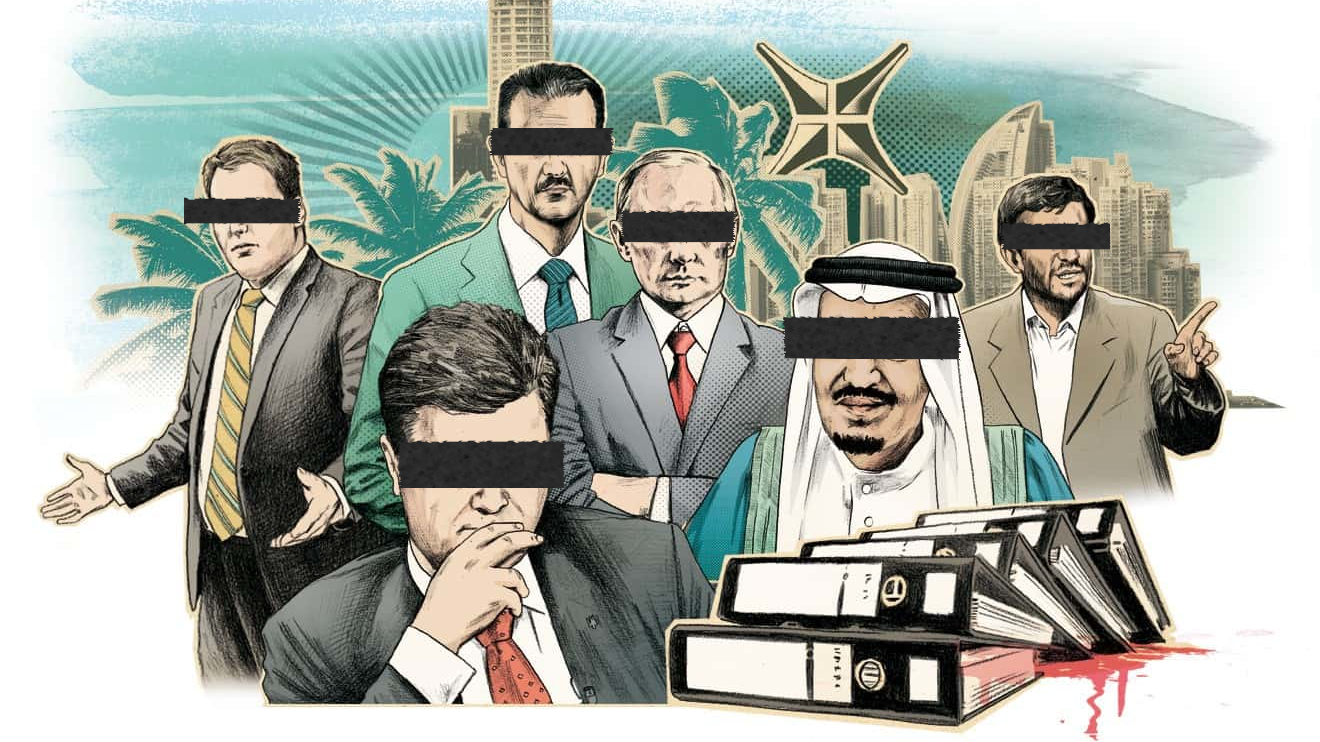
\includegraphics[
                        width = 1\paperwidth,
                        height = 1\paperheight,
                        keepaspectratio
                    ]{images/panamapapers/coverpanamapapershidden.jpg}
                };
            \end{pgfonlayer}
        \end{tikzpicture}
        \note[item]{
            Qualcuno saprebbe riconoscere chi sono le persone in questa slide?
        
            {\color{orange}\textit{wait 5 seconds}}
        }
        \note[item]{
            Vediamolo:
            
            {\color{orange}\textbf{This 00:10}} | {\color{red}\textbf{All 00:10}} | {\color{blue}\textit{Go to next slide}}
        }
    \end{frame}
    
    \begin{frame}{}
        \begin{tikzpicture}[remember picture,overlay]
            \begin{pgfonlayer}{background}
                \node[anchor=south east,outer sep=0pt,inner sep=0pt] at ($(current page.south east) +(-0in,0in)$) {
                    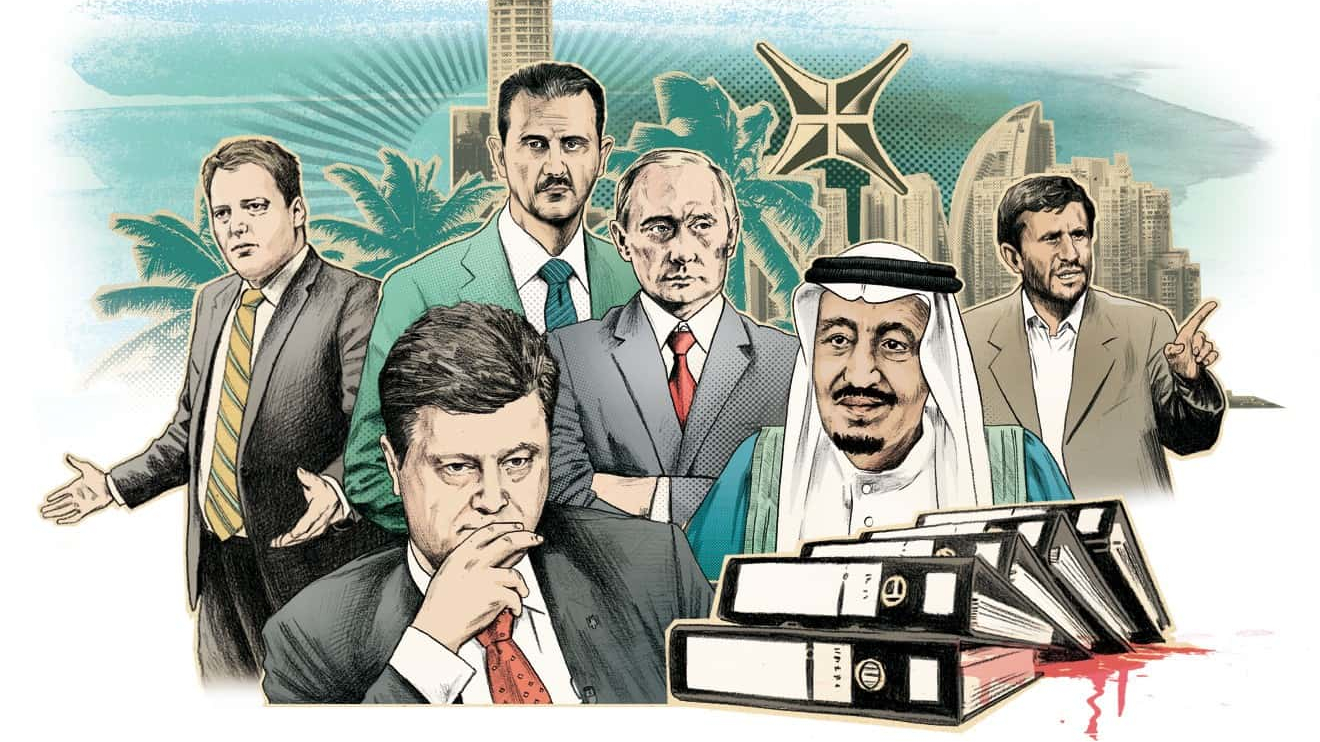
\includegraphics[
                        width = 1\paperwidth,
                        height = 1\paperheight,
                        keepaspectratio
                    ]{images/panamapapers/coverpanamapapersrevealed.jpg}
                };
            \end{pgfonlayer}
        \end{tikzpicture}
        \note[item]{
            Putin, Assad, Poroshenko, il re Salman, Ahmadinejad...
            
            Tutti politici di altissimo livello...
        }
        \note[item]{
            che apparvero nel...
            
            {\color{orange}\textbf{This 00:10}} | {\color{red}\textbf{All 00:20}} | {\color{blue}\textit{Go to next slide}}
        }
    \end{frame}
    
    \begin{frame}{}
        \begin{tikzpicture}[remember picture,overlay]
            \begin{pgfonlayer}{background}
                \node[anchor=south east,outer sep=0pt,inner sep=0pt] at ($(current page.south east) +(-0in,0in)$) {
                    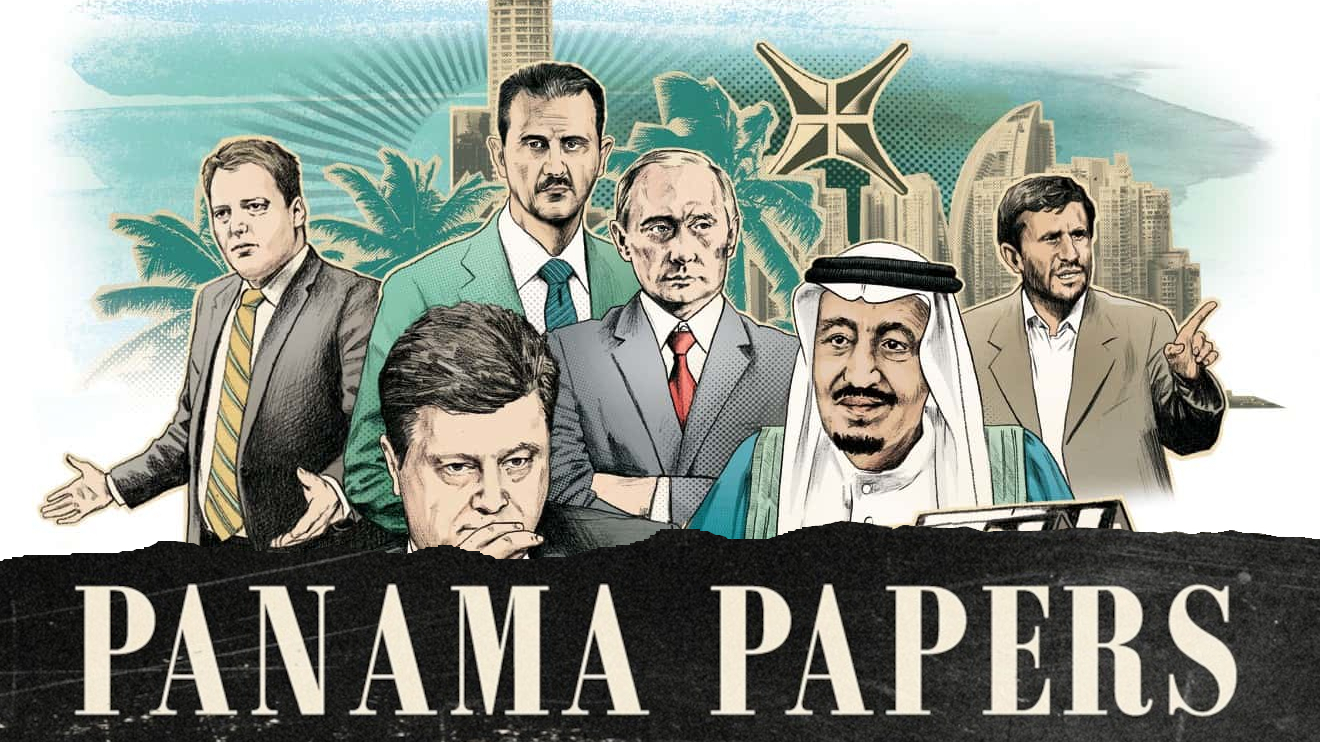
\includegraphics[
                        width = 1\paperwidth,
                        height = 1\paperheight,
                        keepaspectratio
                    ]{images/panamapapers/coverpanamapapersrevealedtitled.jpg}
                };
            \end{pgfonlayer}
        \end{tikzpicture}
        \note[item]{
            ...Panama Papers leak.
        }
        \note[item]{
            Ma cosa erano i Panama Papers?
            
            {\color{orange}\textbf{This 00:15}} | {\color{red}\textbf{All 00:35}} | {\color{blue}\textit{Go to next slide}}
        }
    \end{frame}
    
    \begin{frame}{}
        \begin{tikzpicture}[remember picture,overlay]
            \begin{pgfonlayer}{background}
                \node[anchor=south east,outer sep=0pt,inner sep=0pt] at ($(current page.south east) +(-0in,0in)$) {
                    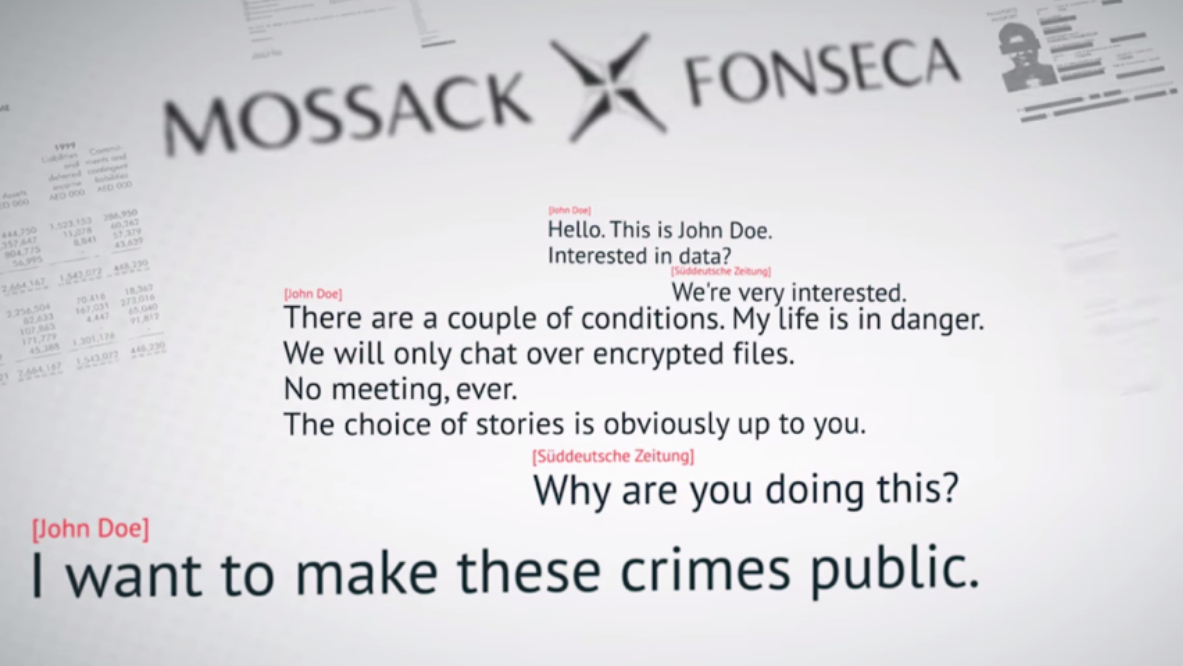
\includegraphics[
                        width = 1\paperwidth,
                        height = 1\paperheight,
                        keepaspectratio
                    ]{images/panamapapers/informer.jpg}
                };
            \end{pgfonlayer}
        \end{tikzpicture}
        \note[item]{
            \begin{itemize}
                \item In aprile 2016,
                \item grazie ad un informatore ...
            \end{itemize}
            
            {\color{orange}\textbf{This 00:5}} | {\color{red}\textbf{All 00:40}} | {\color{blue}\textit{Go to next slide}}
        }
    \end{frame}
    
    \begin{frame}{}
        \begin{tikzpicture}[remember picture,overlay]
            \begin{pgfonlayer}{background}
                \node[anchor=south east,outer sep=0pt,inner sep=0pt] at ($(current page.south east) +(-0in,0in)$) {
                    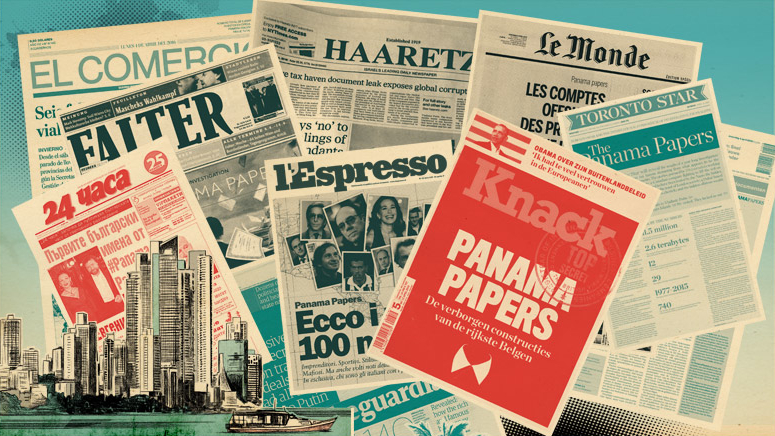
\includegraphics[
                        width = 1\paperwidth,
                        height = 1\paperheight,
                        keepaspectratio
                    ]{images/panamapapers/newspapers.jpg}
                };
            \end{pgfonlayer}
        \end{tikzpicture}
        \note[item]{
            \begin{itemize}
                \item ... l'inchiesta di 307 giornalisti da 76 paesi ha portato alla luce documenti e informazioni
                \item su migliardi di denaro dirottati da studi legali internazionali e banche verso paradisi fiscali
                \item per conto di...
            \end{itemize}
            
            {\color{orange}\textbf{This 00:15}} | {\color{red}\textbf{All 00:55}} | {\color{blue}\textit{Go to next slide}}
        }
    \end{frame}
    
    \begin{frame}{}
        \begin{tikzpicture}[remember picture,overlay]
            \begin{pgfonlayer}{background}
                \node[anchor=south east,outer sep=0pt,inner sep=0pt] at ($(current page.south east) +(-0in,0in)$) {
                    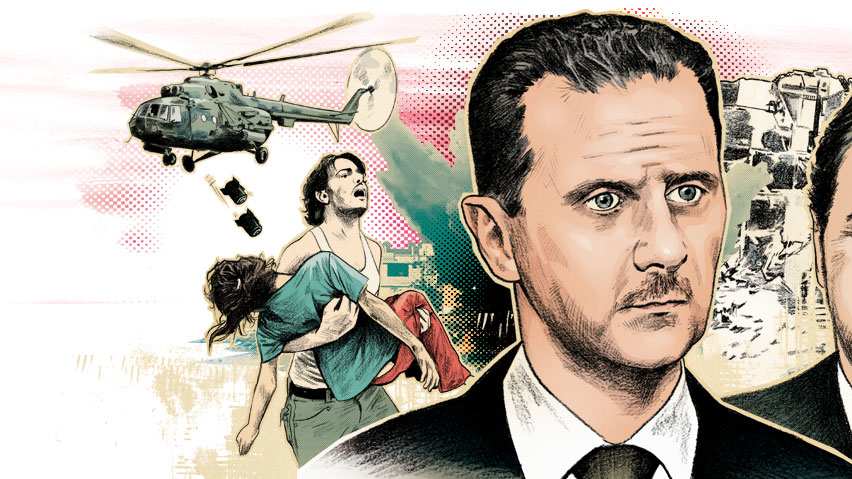
\includegraphics[
                        width = 1\paperwidth,
                        height = 1\paperheight,
                        keepaspectratio
                    ]{images/panamapapers/Assad.jpg}
                };
            \end{pgfonlayer}
        \end{tikzpicture}
        \note[item]{
            ... leader politici, criminali ...
            
            {\color{orange}\textbf{This 00:05}} | {\color{red}\textbf{All 01:00}} | {\color{blue}\textit{Go to next slide}}
        }
    \end{frame}
    
    \begin{frame}{}
        \begin{tikzpicture}[remember picture,overlay]
            \begin{pgfonlayer}{background}
                \node[anchor=south east,outer sep=0pt,inner sep=0pt] at ($(current page.south east) +(-0in,0in)$) {
                    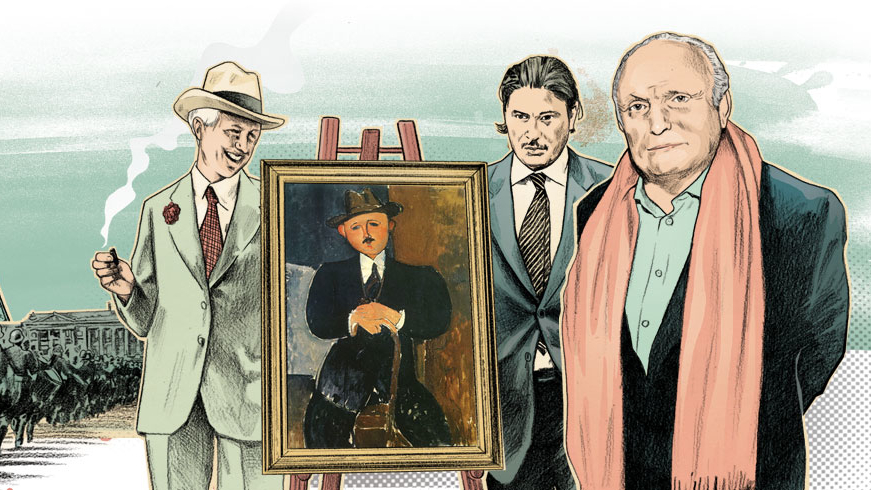
\includegraphics[
                        width = 1\paperwidth,
                        height = 1\paperheight,
                        keepaspectratio
                    ]{images/panamapapers/art.jpg}
                };
            \end{pgfonlayer}
        \end{tikzpicture}
        \note[item]{
            ... funzionari d'intelligence, artisti ...
            
            {\color{orange}\textbf{This 00:05}} | {\color{red}\textbf{All 01:05}} | {\color{blue}\textit{Go to next slide}}
        }
    \end{frame}
    
    \begin{frame}{}
        \begin{tikzpicture}[remember picture,overlay]
            \begin{pgfonlayer}{background}
                \node[anchor=south east,outer sep=0pt,inner sep=0pt] at ($(current page.south east) +(-0in,0in)$) {
                    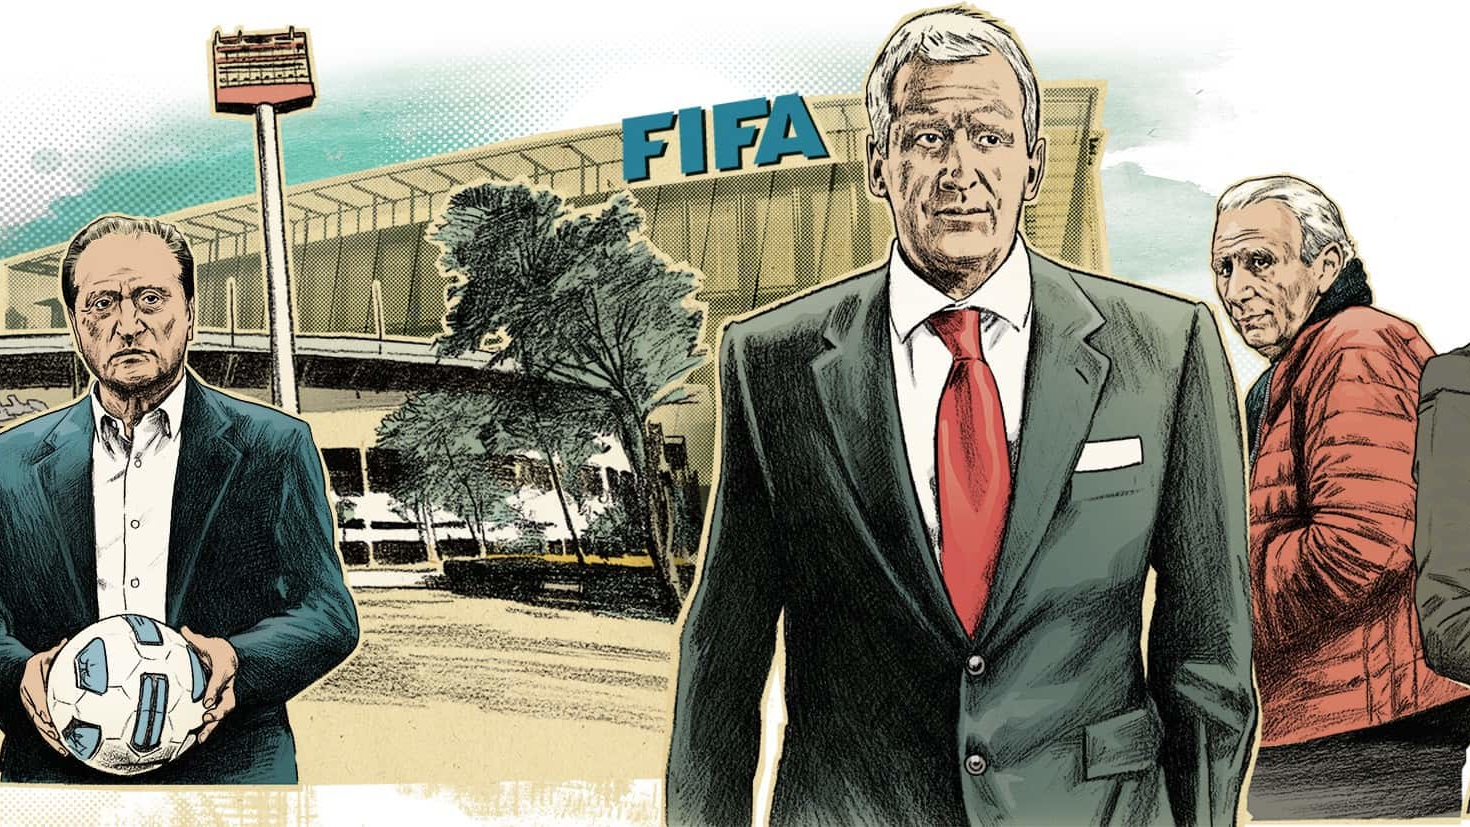
\includegraphics[
                        width = 1\paperwidth,
                        height = 1\paperheight,
                        keepaspectratio
                    ]{images/panamapapers/FIFA1.jpg}
                };
            \end{pgfonlayer}
        \end{tikzpicture}
        \note[item]{
            ... VIP dello sport ...
            
            {\color{orange}\textbf{This 00:05}} | {\color{red}\textbf{All 01:10}} | {\color{blue}\textit{Go to next slide}}
        }
    \end{frame}
    
    \begin{frame}{}
        \begin{tikzpicture}[remember picture,overlay]
            \begin{pgfonlayer}{background}
                \node[anchor=south east,outer sep=0pt,inner sep=0pt] at ($(current page.south east) +(-0in,0in)$) {
                    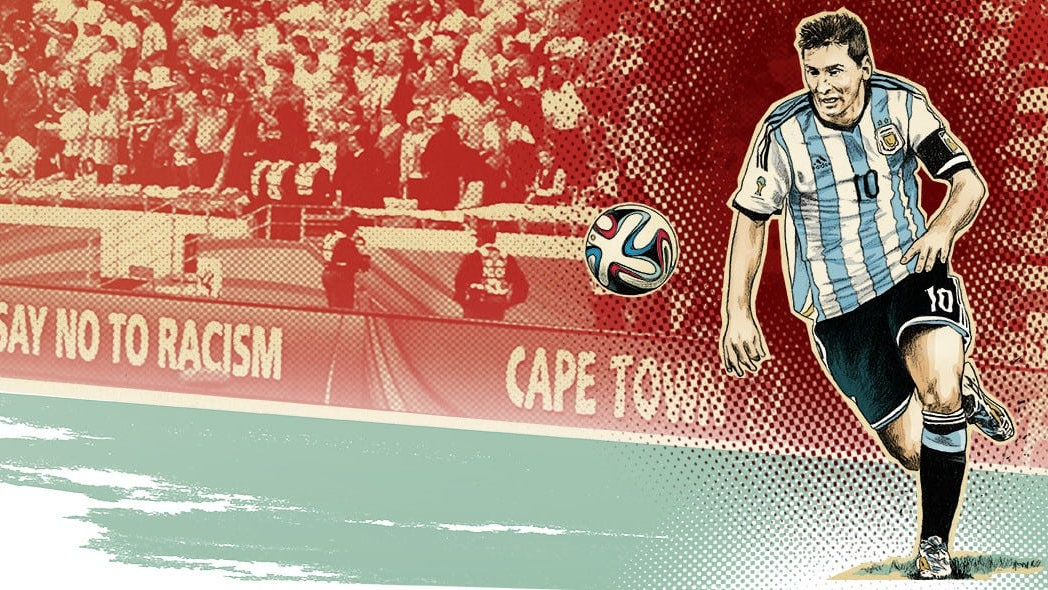
\includegraphics[
                        width = 1\paperwidth,
                        height = 1\paperheight,
                        keepaspectratio
                    ]{images/panamapapers/Messi.jpg}
                };
            \end{pgfonlayer}
        \end{tikzpicture}
        \note[item]{
            ... e dello spettacolo.
            
            {\color{orange}\textit{wait 5 seconds}}
        }
        \note[item]{
            \begin{itemize}
                \item Quanto era grande il dataset leakato?
                \item ... come erano strutturati i dati?
            \end{itemize}
            
            {\color{orange}\textbf{This 00:15}} | {\color{red}\textbf{All 01:25}} | {\color{blue}\textit{Go to next slide}}
        }
    \end{frame}
    
    \begin{frame}{}
        \begin{tikzpicture}[remember picture,overlay]
            \begin{pgfonlayer}{background}
                \node[anchor=south east,outer sep=0pt,inner sep=0pt] at ($(current page.south east) +(-0in,0in)$) {
                    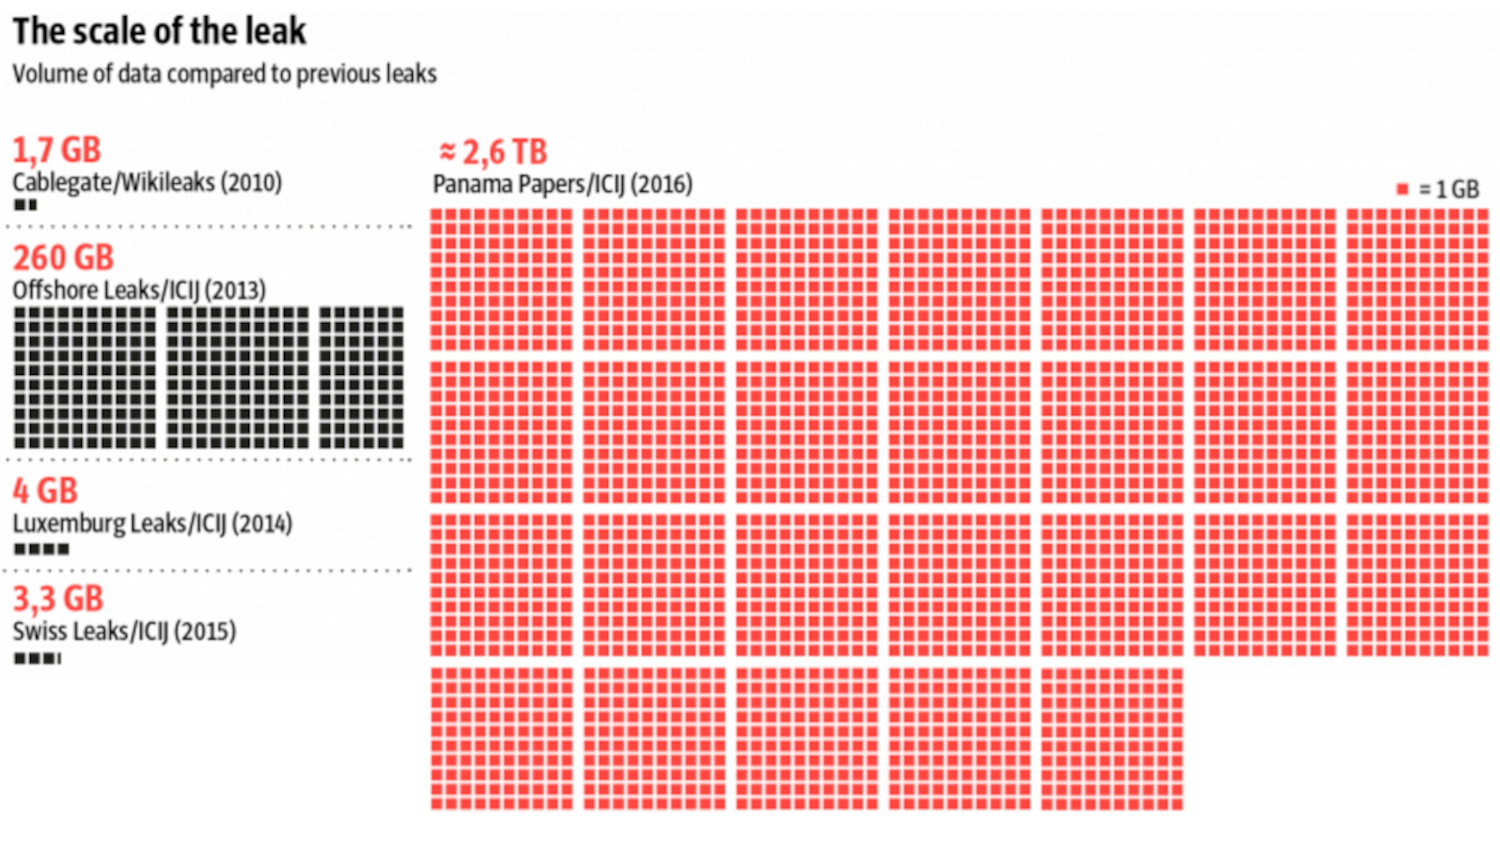
\includegraphics[
                        width = 1\paperwidth,
                        height = 1\paperheight,
                        keepaspectratio
                    ]{images/panamapapers/datasetsizenew.jpg}
                };
            \end{pgfonlayer}
        \end{tikzpicture}
        \note[item]{
            Il leak era di dimensione 2.6 TB, 1500 volte più grande del Cablegate del 2010 di Wikileaks.
            
            {\color{orange}\textbf{This 00:10}} | {\color{red}\textbf{All 01:35}} | {\color{blue}\textit{Go to next slide}}
        }
    \end{frame}
    
    \begin{frame}{}
        \begin{tikzpicture}[remember picture,overlay]
            \begin{pgfonlayer}{background}
                \node[anchor=south east,outer sep=0pt,inner sep=0pt] at ($(current page.south east) +(-0in,0in)$) {
                    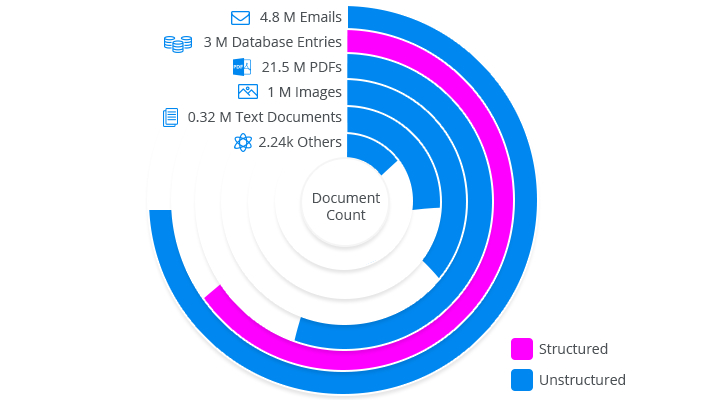
\includegraphics[
                        width = 1\paperwidth,
                        height = 1\paperheight,
                        keepaspectratio
                    ]{images/panamapapers/datatypes.jpg}
                };
            \end{pgfonlayer}
        \end{tikzpicture}
        \note[item]{
            La maggior parte dei dati erano non strutturati, sotto forma di emails, immagini e files PDF inviati.
            
            {\color{orange}\textbf{This 00:10}} | {\color{red}\textbf{All 01:45}} | {\color{blue}\textit{Go to next slide}}
        }
    \end{frame}
    
    \begin{frame}{}
        \begin{tikzpicture}[remember picture,overlay]
            \begin{pgfonlayer}{background}
                \node[anchor=south east,outer sep=0pt,inner sep=0pt] at ($(current page.south east) +(-0in,0in)$) {
                    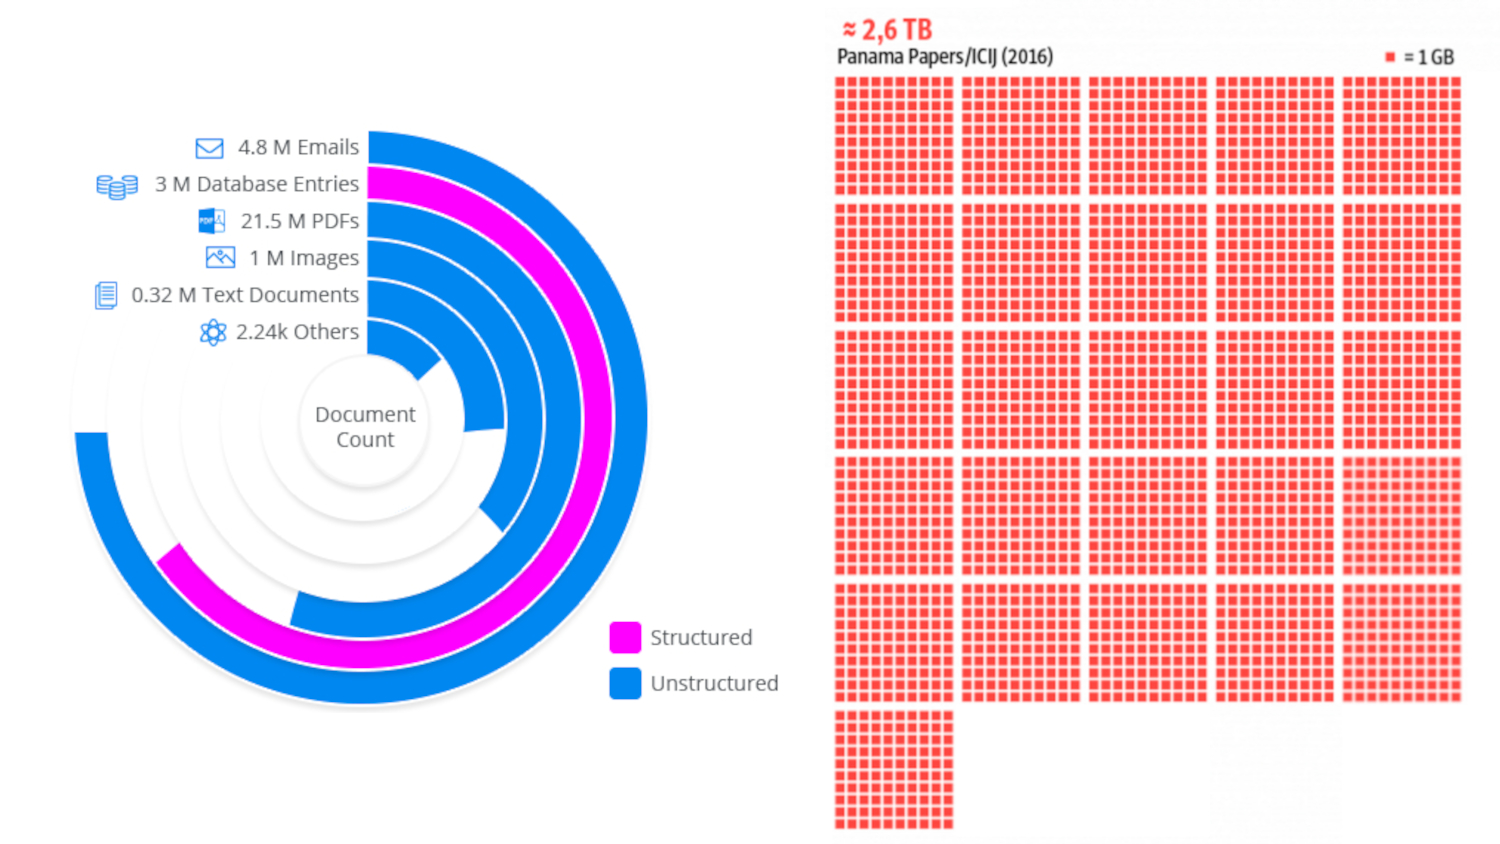
\includegraphics[
                        width = 1\paperwidth,
                        height = 1\paperheight,
                        keepaspectratio
                    ]{images/panamapapers/datasetsizeandtypes.jpg}
                };
            \end{pgfonlayer}
        \end{tikzpicture}
        \note[item]{
            \begin{itemize}
                \item Una domanda sorge spontanea:
                \item Come si può indagare su un dataset così immenso
                \item e in gran parte fatto di dati non strutturati?
            \end{itemize}
            
            {\color{orange}\textbf{This 00:15}} | {\color{red}\textbf{All 02:00}} | {\color{blue}\textit{Go to next slide}}
        }
    \end{frame}
    
    \begin{frame}{}
        \begin{tikzpicture}[remember picture,overlay]
            \begin{pgfonlayer}{background}
                \node[anchor=south east,outer sep=0pt,inner sep=0pt] at ($(current page.south east) +(-0in,0in)$) {
                    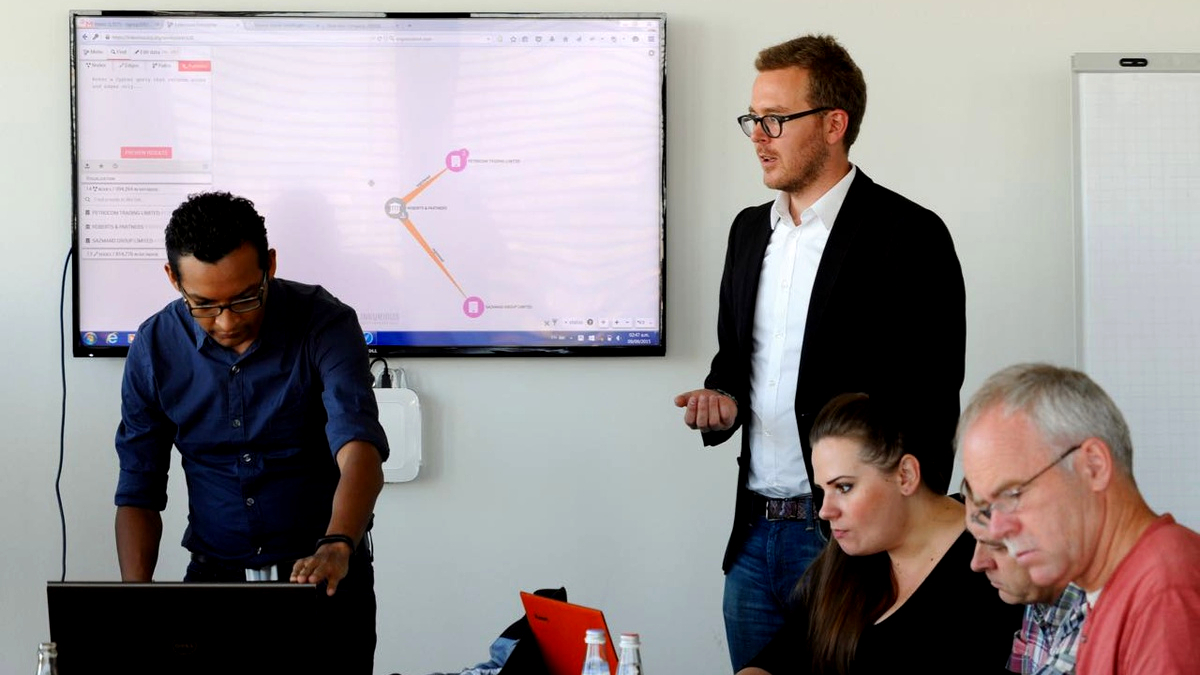
\includegraphics[
                        width = 1\paperwidth,
                        height = 1\paperheight,
                        keepaspectratio
                    ]{images/panamapapers/team.jpg}
                };
            \end{pgfonlayer}
        \end{tikzpicture}
        \note[item]{
            Loro, un team composto da giornalisti investigativi ed esperti di database a grafi ce l'hanno fatta.
            
            {\color{orange}\textbf{This 00:10}} | {\color{red}\textbf{All 02:10}} | {\color{blue}\textit{Go to next slide}}
        }
    \end{frame}
    
    \begin{frame}{}
        \begin{tikzpicture}[remember picture,overlay]
            \begin{pgfonlayer}{background}
                \node[anchor=south east,outer sep=0pt,inner sep=0pt] at ($(current page.south east) +(-0in,0in)$) {
                    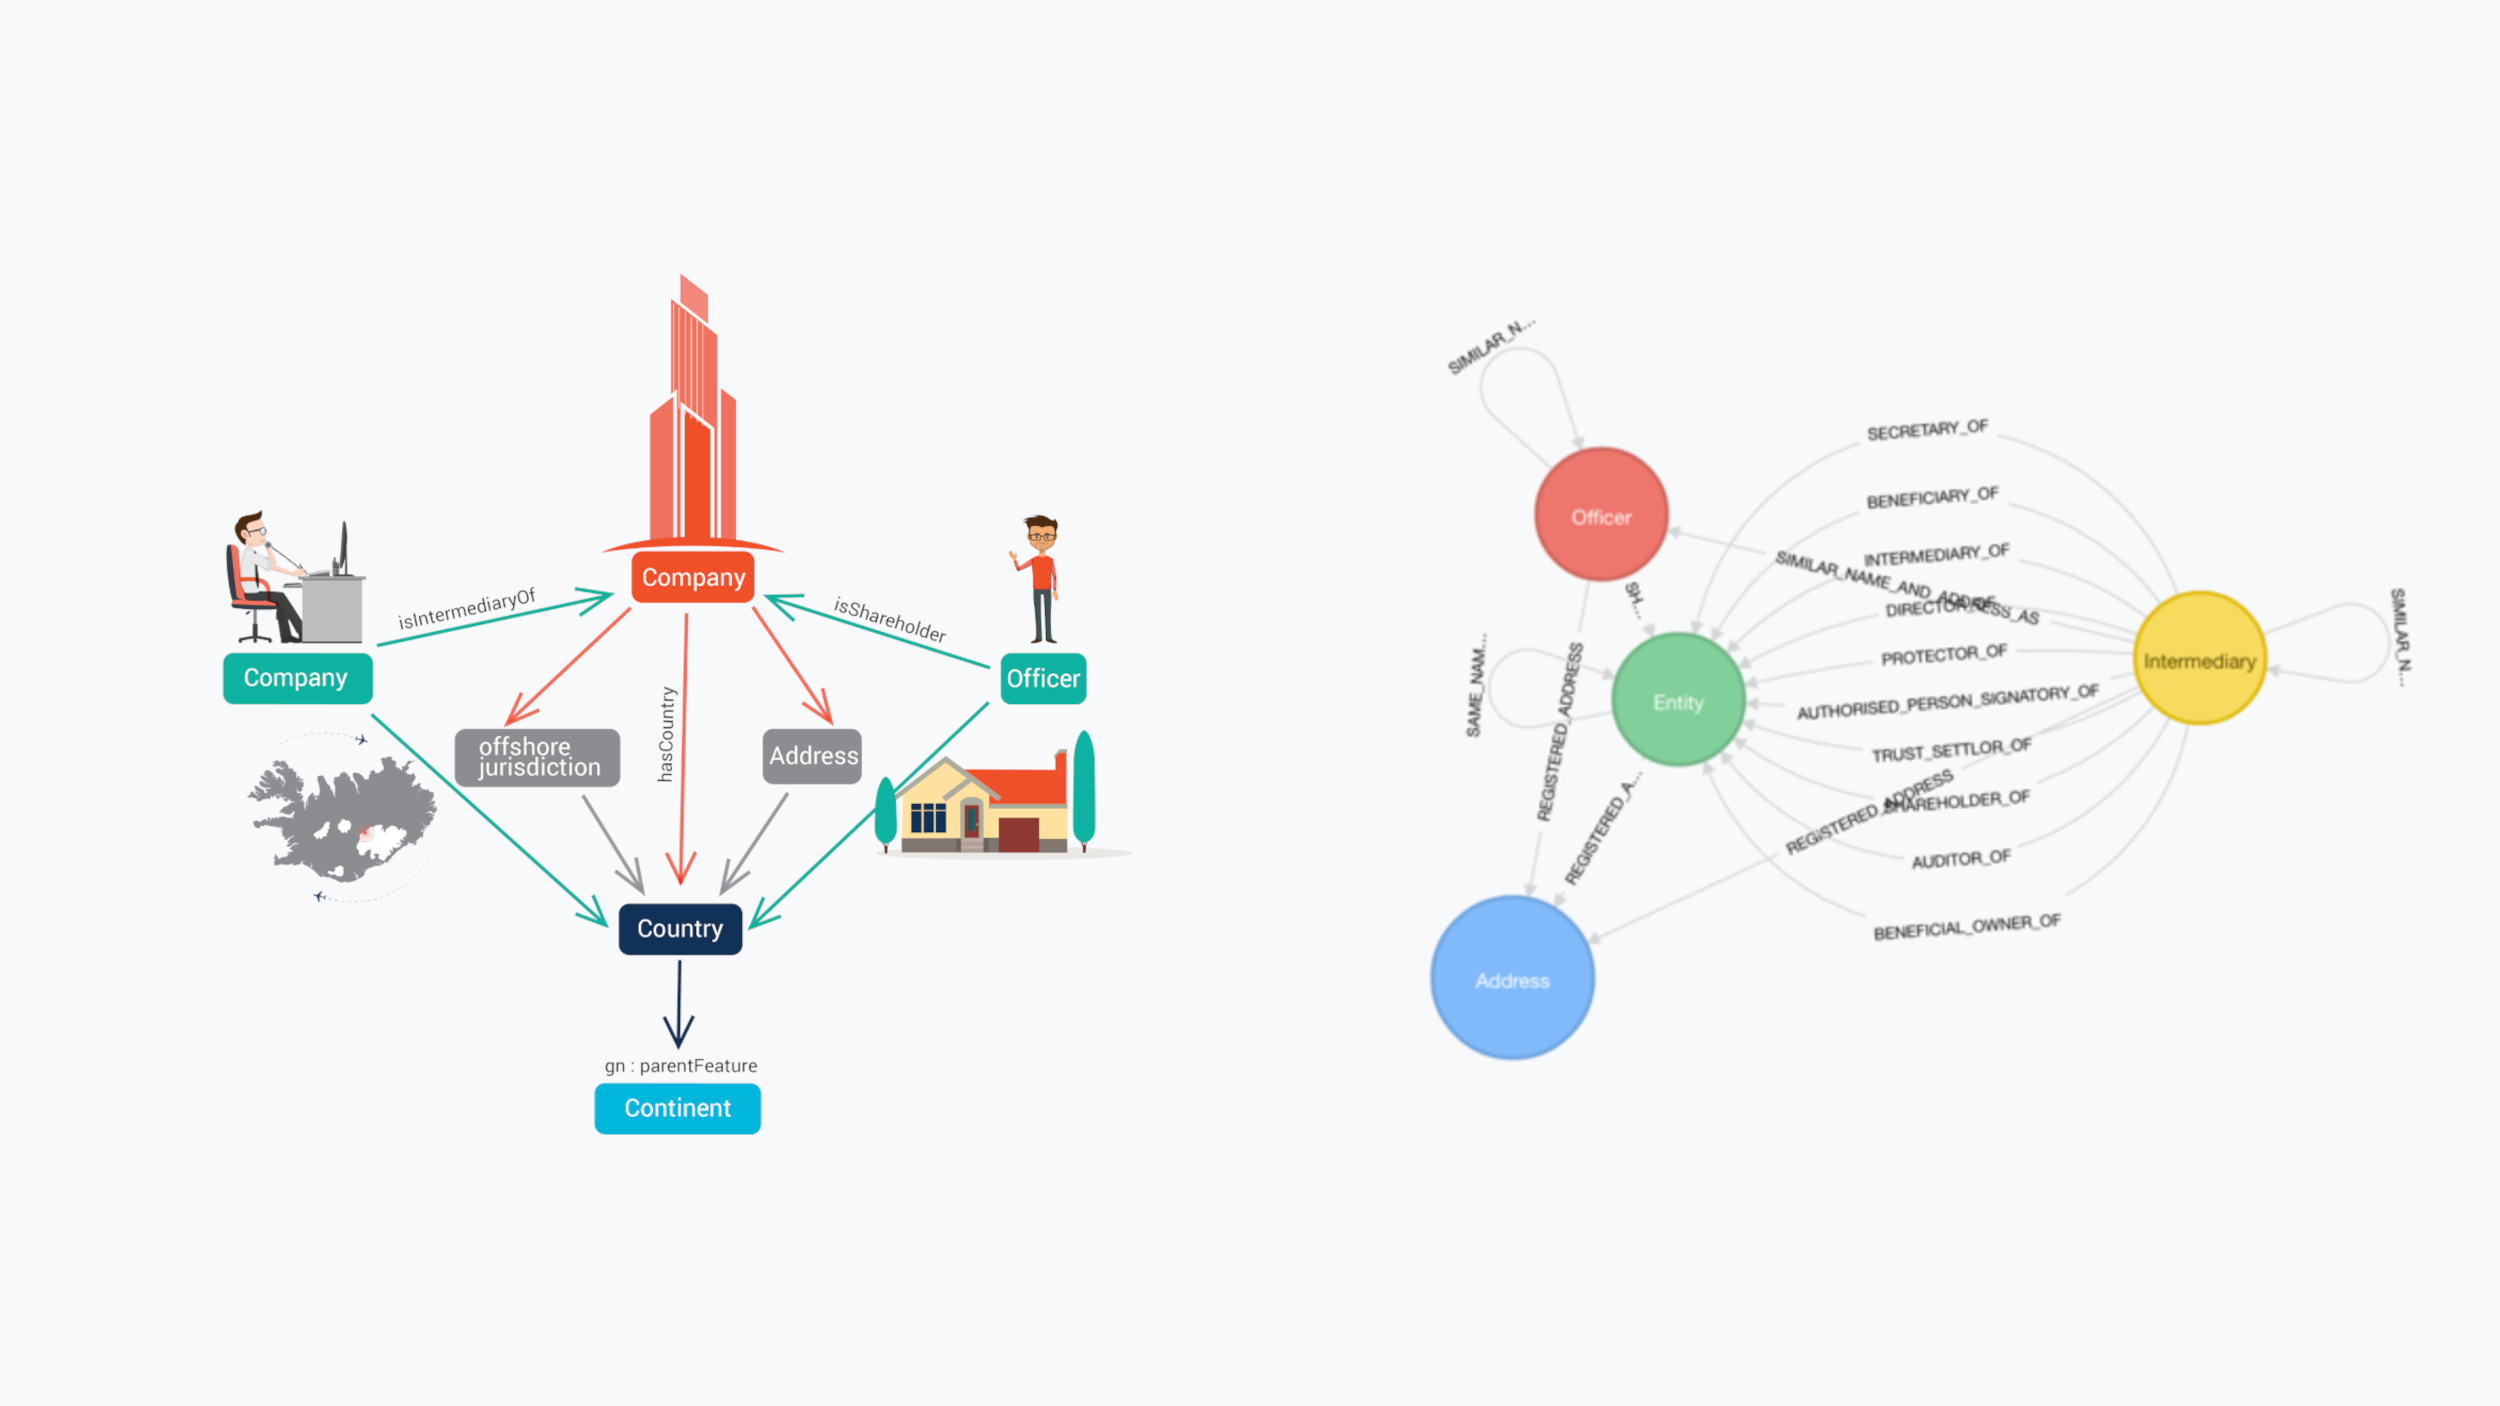
\includegraphics[
                        width = 1\paperwidth,
                        height = 1\paperheight,
                        keepaspectratio
                    ]{images/panamapapers/graphsmall.jpg}
                };
            \end{pgfonlayer}
        \end{tikzpicture}
        \note[item]{
            Facendo buon uso delle relazioni che derivano da dati interconnessi (ad esempio le mail, le dipendenze tra le entità) ...
            
            {\color{orange}\textbf{This 00:10}} | {\color{red}\textbf{All 02:20}} | {\color{blue}\textit{Go to next slide}}
        }
    \end{frame}
    
    \begin{frame}{}
        \begin{tikzpicture}[remember picture,overlay]
            \begin{pgfonlayer}{background}
                \node[anchor=south east,outer sep=0pt,inner sep=0pt] at ($(current page.south east) +(-0in,0in)$) {
                    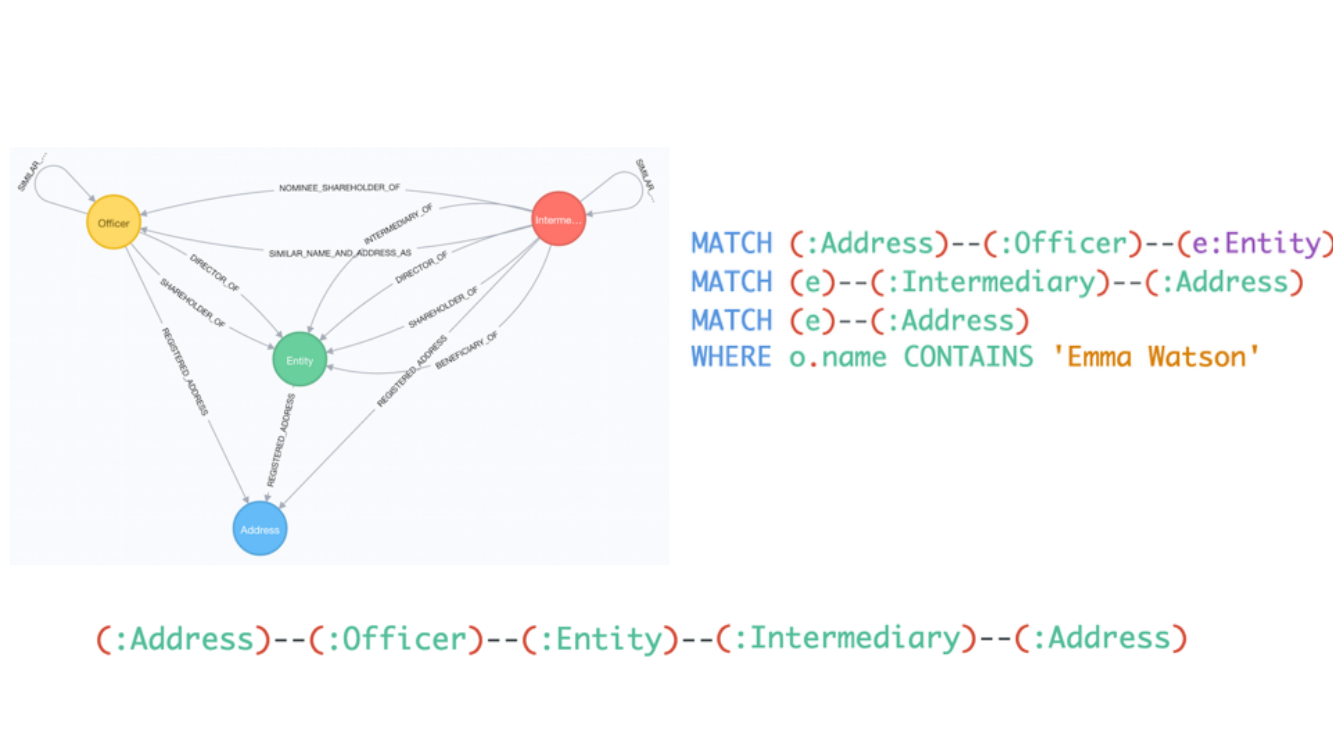
\includegraphics[
                        width = 1\paperwidth,
                        height = 1\paperheight,
                        keepaspectratio
                    ]{images/panamapapers/neo4jcypher.jpg}
                };
            \end{pgfonlayer}
        \end{tikzpicture}
        \note[item]{
            \begin{itemize}
                \item ... e di nuove tecnologie (come i database a grafi),
                \item hanno generato grafi con nodi rappresentanti le entità coinvolte
                \item e archi rappresentanti le connessioni tra loro,
            \end{itemize}
            
            {\color{orange}\textbf{This 00:15}} | {\color{red}\textbf{All 02:35}} | {\color{blue}\textit{Go to next slide}}
        }
    \end{frame}
    
    \begin{frame}{}
        \begin{tikzpicture}[remember picture,overlay]
            \begin{pgfonlayer}{background}
                \node[anchor=south east,outer sep=0pt,inner sep=0pt] at ($(current page.south east) +(-0in,0in)$) {
                    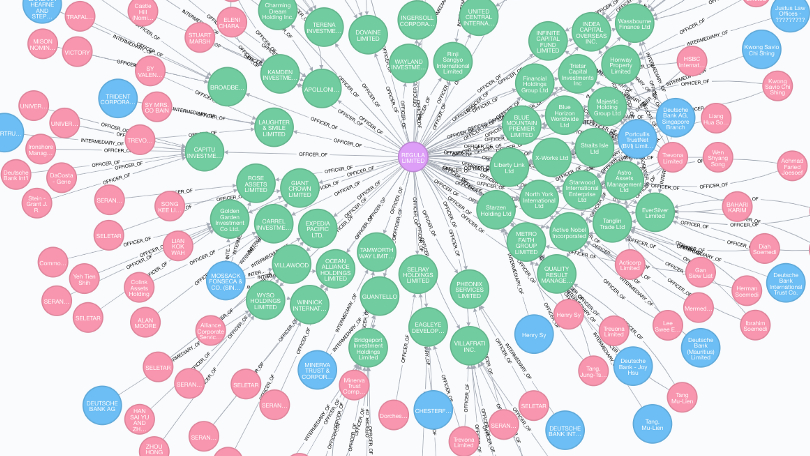
\includegraphics[
                        width = 1\paperwidth,
                        height = 1\paperheight,
                        keepaspectratio
                    ]{images/panamapapers/graph.jpg}
                };
            \end{pgfonlayer}
        \end{tikzpicture}
        \note[item]{
            \begin{itemize}
                \item il tutto interrogabile
            \end{itemize}
        }
        \note[item]{
            \begin{itemize}
                \item Questo è uno dei più eclatanti esempi a queste dimensioni
                \item dell'utilizzo di database a grafi per svolgere un compito
                \item che altri tipi di database semplicemente non potevano fare
                \item (almeno i tempi di interrogazione non sarebbero stati umanamente accettabili)
                \item perché non progettati per effettuare visite su grafi con dati non strutturati.
            \end{itemize}
        }
        \note[item]{
            \begin{itemize}
                \item Nel lavoro svolto per la tesi, non si è parlato di Panama Papers.
                \item Ma:
            \end{itemize}
            
            {\color{orange}\textbf{This 00:35}} | {\color{red}\textbf{All 03:10}} | {\color{blue}\textit{Go to next slide}}
        }
    \end{frame}
    
    \begin{frame}[noframenumbering, standout]
        \normalfont
        
        \vspace*{0.75cm}
        \fontsize{26pt}{33pt}\selectfont\textsc{\break\mydocumenttitle}
        
        \begin{columns}[t]
            \column{0.13\textwidth}
            
            \column{0.69\textwidth}
                \vspace*{-1.25cm}
                \begin{center}
                    \Large\normalfont\mydocumentsubtitle
                    
                    \vspace*{0.5cm}
                    \normalsize\textbf{\myauthor}
                \end{center}
                
                    
                %\mydateofpublishing
                
                \begin{tikzpicture}[remember picture,overlay]
                    \begin{pgfonlayer}{background}
                        \node[anchor=south east,outer sep=0pt,inner sep=0pt] at ($(current page.south east) +(-0in,0in)$) {
                            
\includegraphics[
                                width = 0.25\paperwidth
                            ]{images/LogoUniBGwhiterotatedcut.pdf}
                        };
                    \end{pgfonlayer}
                \end{tikzpicture}
                
            \column{0.13\textwidth}
        \end{columns}
        \note[item]{
            \normalfont
            \begin{itemize}
                \item Facendo uso di un database a grafi per il salvataggio
                \item e l'interrogazione di dati di un dataset di 5.6 milioni di pubblicazioni scientifiche accademiche da 2.8 milioni di ricercatori,
                \item applicando al grafo da essi generati un algoritmo di Community Detection,
                \item ovvero, di individuazione delle comunità
                \item sono state individuate 180 mila Communities.
                \item Inoltre, è stata sviluppata una Full-Stack Web Application per visualizzare queste comunità di collaborazione.
            \end{itemize}
        }
        \note[item]{
            \normalfont
            Più in dettaglio:
            
            {\color{orange}\textbf{This 00:40}} | {\color{red}\textbf{All 03:50}} | {\color{blue}\textit{Go to next slide}}
        }
    \end{frame}
    \stepcounter{framenumber}
    
    \begin{frame}{The work done}
        \begin{enumerate}
            \item \textbf{Literature review} of graph theory, graph databases and clustering algorithms.
            \item \texttt{dblp.org} \textbf{Dataset download, conversion \& import} in ArangoDB Graph DBMS.
            \item \textbf{Data transformations} to obtain vertices, edges and the complete graph.
            \item \textbf{Community Detection Algorithm application} on the graph for clustering.
            \item \textbf{Web Application development} to display the results of the clustering.
        \end{enumerate}
        
        \note[item]{
            \begin{itemize}
                \item \footnotesize È stata fatta una consultazione in letteratura dei concetti base di teoria dei grafi,
                \item \footnotesize delle varie caratteristiche dei database a grafi
                \item \footnotesize e degli algoritmi per l'individuazione delle communities in grafi.
            \end{itemize}
        }
        \note[item]{
            \begin{itemize}
                \item \footnotesize Poi è stato scaricato il dataset da dblp.org, è stato convertito
                \item \footnotesize e importato su ArangoDB, il graph database management system scelto.
            \end{itemize}
        }
        \note[item]{
            \begin{itemize}
                \item \footnotesize Le collezioni di dati sono state sottoposte a trasformazioni per ottenere vertici,
                \item \footnotesize archi e da questi il grafo completo dell'intero dataset.
            \end{itemize}
        }
        \note[item]{
            \begin{itemize}
                \item \footnotesize Su tale grafo poi è stato applicato un Label Propagation Community Detection Algorithm,
                \item \footnotesize ovvero un algoritmo a propagazione di etichette per l'individuazione delle comunità di collaborazione scientifica.
            \end{itemize}
        }
        \note[item]{
            \begin{itemize}
                \item \footnotesize In fine, è stata sviluppata una Web Application per visualizzare le communities individuate.
            \end{itemize}
        }
        \note[item]{
            \footnotesize Vediamoli uno ad uno...
            
            \large {\color{orange}\textbf{This 00:50}} | {\color{red}\textbf{All 04:40}} | {\color{blue}\textit{Go to next slide}}
        }
    \end{frame}
    
    \begin{frame}{Graph databases}
        \centering
        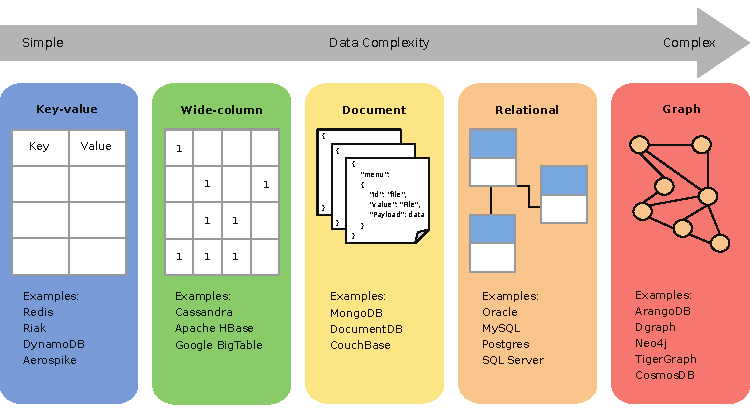
\includegraphics[width = 0.78\paperwidth, height = 0.78\paperheight, keepaspectratio]{images/BechbergerPerryman2020page8.pdf}
        
        \note[item]{
            \begin{itemize}
                \item ... più i dati sono interconnessi e strutturati in modo complesso,
                \item più fa senso usare database a grafi
            \end{itemize}
        }
        \note[item]{
            \begin{itemize}
                \item Inoltre se i nested JOINs da fare durante un'interrogazione sono più di 3 livelli di profondità,
            \end{itemize}
            
            {\color{orange}\textbf{This 00:15}} | {\color{red}\textbf{All 04:55}} | {\color{blue}\textit{Go to next slide}}
        }
    \end{frame}
    
    \begin{frame}{}
        \begin{tikzpicture}[remember picture,overlay]
            \begin{pgfonlayer}{background}
                \node[anchor=south east,outer sep=0pt,inner sep=0pt] at ($(current page.south east) +(-0in,0in)$) {
                    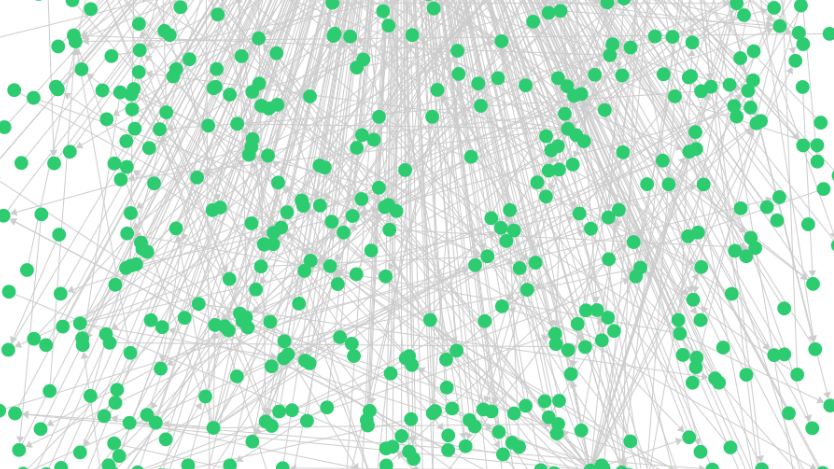
\includegraphics[
                        width = 1\paperwidth,
                        height = 1\paperheight,
                        keepaspectratio
                    ]{images/PregelDetectedCommunityOtherVerticesResultcut.jpg}
                };
            \end{pgfonlayer}
        \end{tikzpicture}
        \note[item]{
            \begin{itemize}
                \item ovverò, in termini di grafi, se bisogna fare più di 3 salti di attraversamento degli archi,
                \item allora i tempi di interrogazione usando database tradizionali diventano proibitivi.
            \end{itemize}
        }
        \note[item]{
            \begin{itemize}
                \item Dunque, vediamo ora concretamente cosa è stato fatto.
            \end{itemize}
            
            {\color{orange}\textbf{This 00:20}} | {\color{red}\textbf{All 05:15}} | {\color{blue}\textit{Go to next slide}}
        }
    \end{frame}
    
    \begin{frame}{Le macchine}
        \begin{tikzpicture}[remember picture,overlay]
            \begin{pgfonlayer}{background}
                \node[anchor=south east,outer sep=0pt,inner sep=0pt] at ($(current page.south east) +(-0in,0in)$) {
                    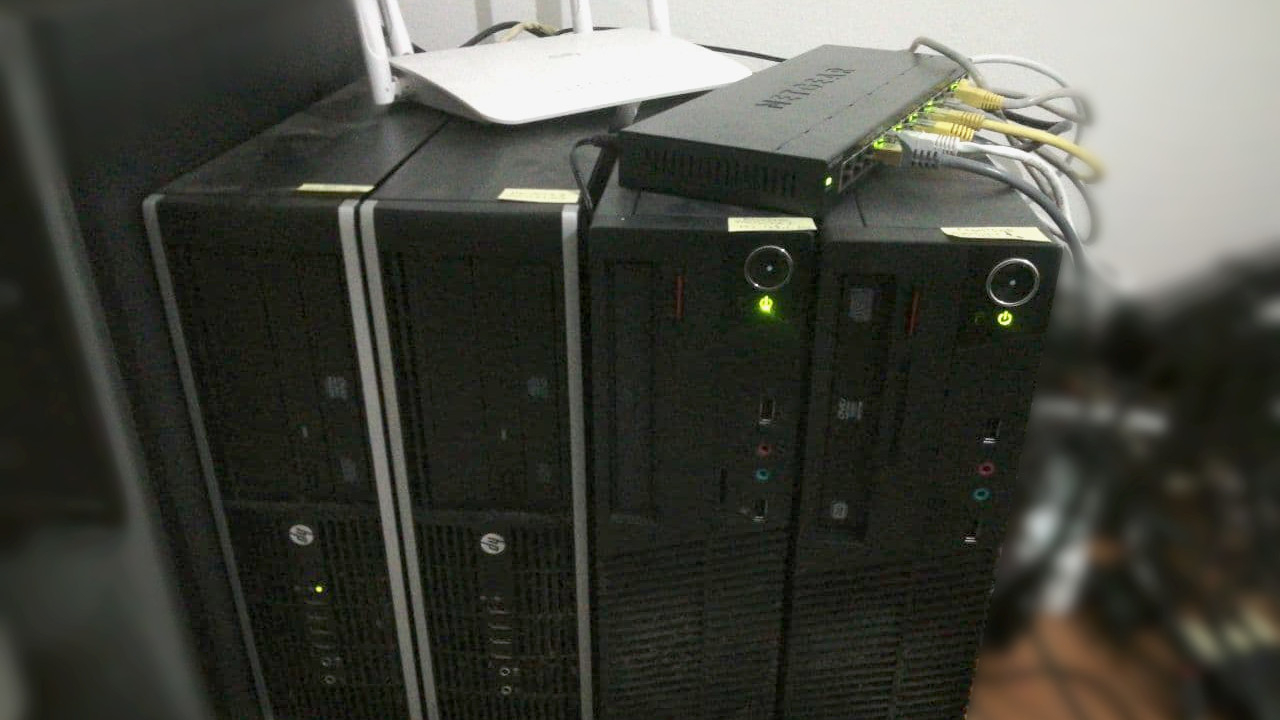
\includegraphics[
                        width = 1\paperwidth,
                        height = 1\paperheight,
                        keepaspectratio
                    ]{images/machinesphotocut.jpg}
                };
            \end{pgfonlayer}
        \end{tikzpicture}
        \note[item]{
            \begin{itemize}
                \item Al fine di hostare il database,
                \item servire l'API della Web Application
                \item e l'interfaccia lato frontend del sito,
                \item 3 macchine separate, un router e uno switch sono stati usati.
                \item La quarta macchina è stata usata a scopi di sviluppo e accesso remoto.
            \end{itemize}
        }
        \note[item]{
            \begin{itemize}
                \item Una volta installato i sistemi operativi sulle varie macchine
                \item e ArangoDB sulla macchina scelta come host del database...
            \end{itemize}
            
            {\color{orange}\textbf{This 00:30}} | {\color{red}\textbf{All 05:45}} | {\color{blue}\textit{Go to next slide}}
        }
    \end{frame}
    
    \begin{frame}{The dataset: dblp.org}
        \begin{center}
            \vspace*{-0.1cm}
            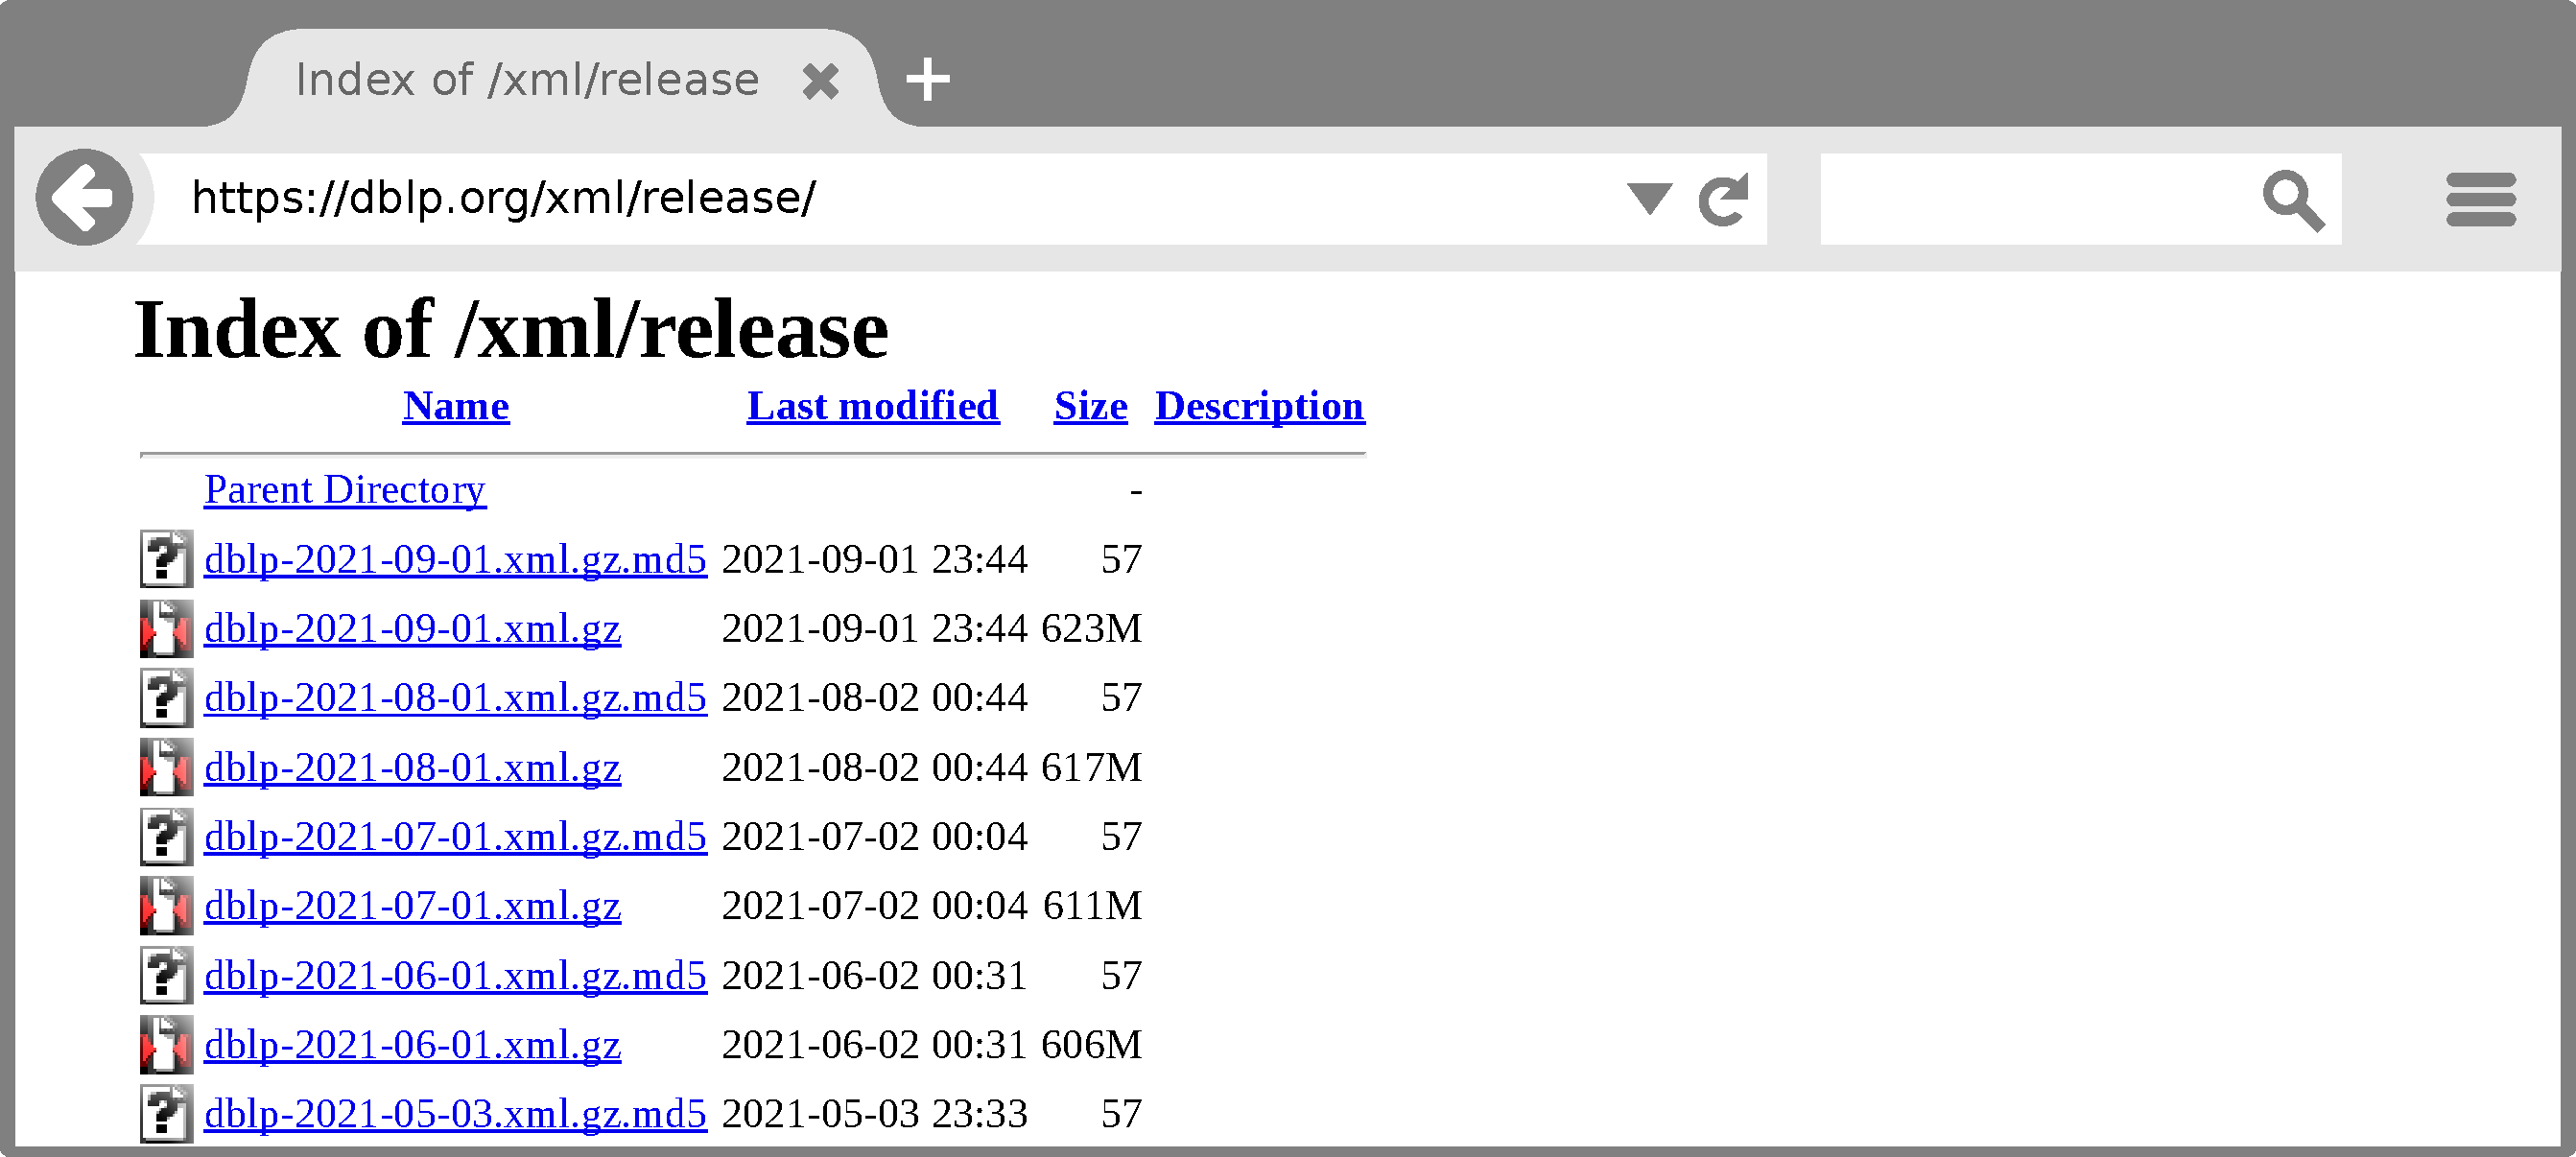
\includegraphics[
                width = 0.70\paperwidth,
                height = 0.70\paperheight,
                keepaspectratio
            ]{images/dblpdatasetdownload.pdf}
        \end{center}
        
        \vspace*{-0.3cm}
        {\color{darkgray}The dataset:}
        \begin{columns}[t]
            \column{.50\textwidth}
                \vspace*{-0.6cm}
                \begin{itemize}
                	\item Compressed archive of 623 MB.
                	\item Once extracted: Single XML file of 3.2 GB.
                \end{itemize}
                
            \column{.50\textwidth}
                \vspace*{-0.6cm}
                \begin{itemize}
                	\item 8.5 million XML entries on publications, authors, journals, institutions, citations etc.
                \end{itemize}
        \end{columns}
        \note[item]{
            \begin{itemize}
                \item si procede al download del dataset dal sito di dblp.org .
                \item Il dataset è fatto da un unico file compresso di dimensione 623 MB.
                \item Una volta estratto, il singolo file XML è di 3.2 GB
                \item e contiene circa 8 millioni e mezzo di voci XML su autori,
                \item publicazioni, affiliazioni, citazioni, journals e così via.
            \end{itemize}
        }
        \note[item]{
            \begin{itemize}
                \item Sicuramente i dati non possono essere importati nel database così
                \item perché ArangoDB richiede che essi siano in formato line JSON.
                \item Perciò serve convertire le voci XML in righe di line JSON.
            \end{itemize}
        }
        \note[item]{
            \begin{itemize}
                \item Un altro problema è la dimensione da 3.2 GB del file XML,
                \item non molto facile da manipolare.
            \end{itemize}
            
            {\color{orange}\textbf{This 00:40}} | {\color{red}\textbf{All 6:25}} | {\color{blue}\textit{Go to next slide}}
        }
    \end{frame}
    
    \begin{frame}{Data conversion, import and transformations}
        \begin{center}
            \vspace*{-0.1cm}
            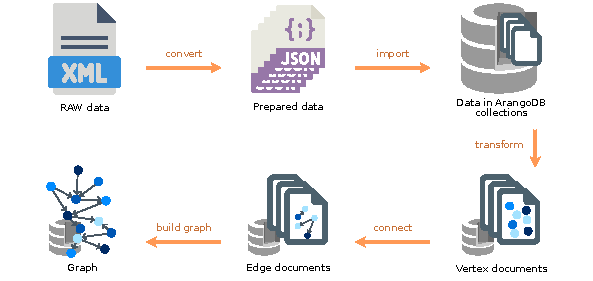
\includegraphics[
                width = 0.7\paperwidth,
                height = 0.7\paperheight,
                keepaspectratio
            ]{images/datatransformations.pdf}
        \end{center}
        
        \vspace*{-0.3cm}
        {\color{darkgray}The steps:}
        \begin{columns}[t]
            \column{.50\textwidth}
                \vspace*{-0.3cm}
                \begin{enumerate}
                	\item \small Conversion from XML to line JSON;
                	\item \small Import in ArangoDB collection;
                \end{enumerate}
                
            \column{.50\textwidth}
                \vspace*{-1.3cm}
                \begin{enumerate}
                    \setcounter{enumi}{2}
                	\item \small Transform imported data to vertex documents;
                	\item \small Link vertices by edges;
                	\item \small Build the graph.
                \end{enumerate}
        \end{columns}
        \note{
            Quindi le operazioni da effettuare per arrivare dai dati grezzi al grafo completo sono:
        }
        \note[item]{
            \begin{itemize}
                \item La suddivisione del file XML in tanti piccoli files
                \item e la conversione di ciascuno di essi in formato line JSON.
            \end{itemize}
        }
        \note[item]{
            L'import dei line JSON in una collection in un database ArangoDB,
        }
        \note[item]{
            \begin{itemize}
                \item La trasformazione dei documenti importati
                \item in modo che possano essere a tutti gli effetti dei vertici di un grafo.
            \end{itemize}
        }
        \note[item]{
            \begin{itemize}
                \item La creazione degli archi tra i vertici usando gli attributi \_from e \_to.
            \end{itemize}
        }
        \note[item]{
            \begin{itemize}
                \item Costruzione del grafo finale con l'insieme delle collezioni dei vertici \item e l'insieme delle collezioni degli archi.
            \end{itemize}
            
            {\color{orange}\textbf{This 00:45}} | {\color{red}\textbf{All 07:10}} | {\color{blue}\textit{Go to next slide}}
        }
    \end{frame}
    
    \begin{frame}{The graph}
        
        \begin{columns}
            \column{.30\textwidth}
                \small
                {\color{darkgray}A subgraph of the obtained final graph:}
            
            \column{.70\textwidth}
                \begin{center}
                    \vspace*{-0.2cm}
                    \hspace*{0.1cm}
                    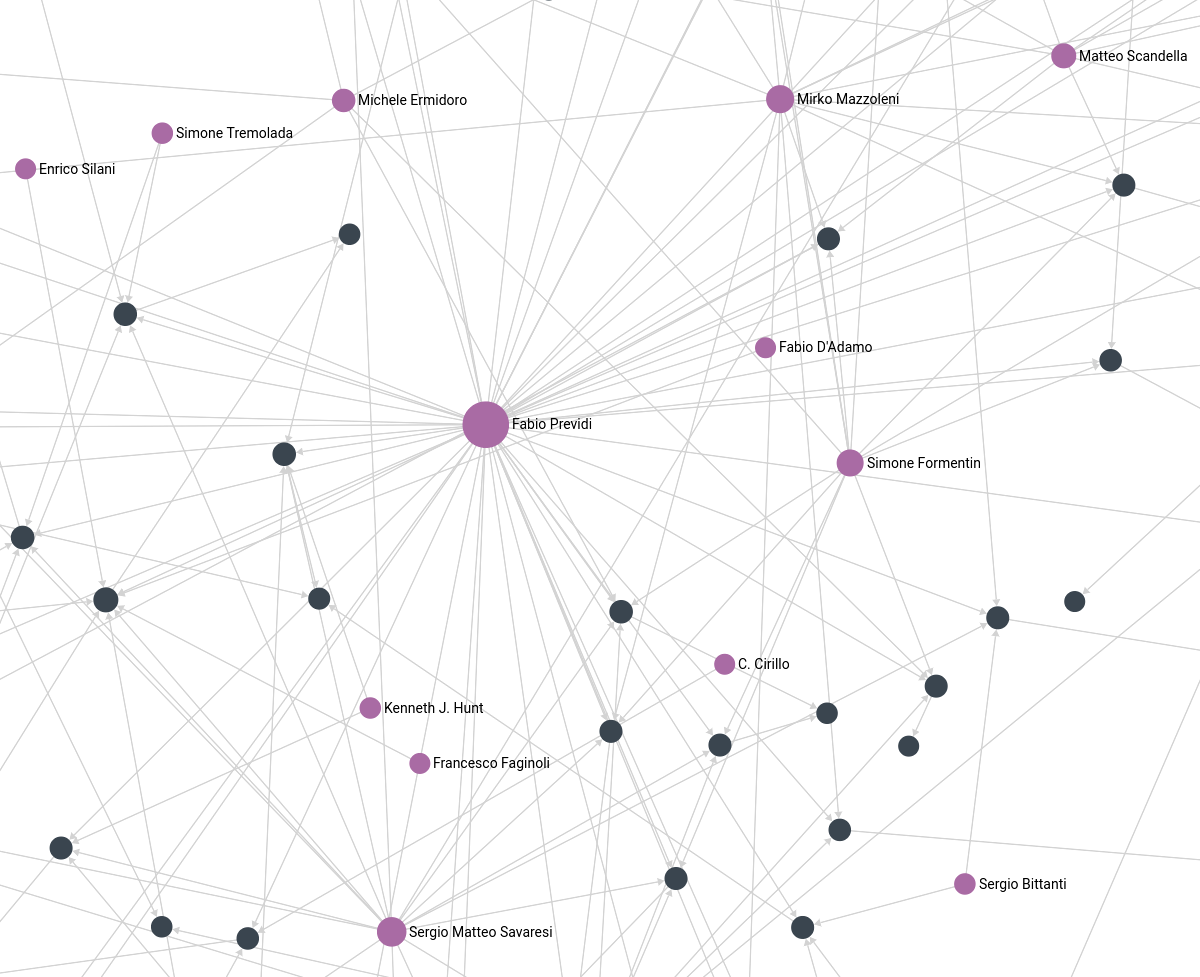
\includegraphics[
                        width = 1\textwidth,
                        height = 0.85\paperheight,
                        keepaspectratio
                    ]{images/SnapshotArangoDBGraphPrevidiMazzolenishort.png}
                \end{center}
        \end{columns}
        \note[item]{
            Questo è un assaggio del grafo finale, o anche una verifica della sua validità.
        }
        \note[item]{
            Il grafo finale è composto dall'insieme di tutti i vertici del dataset e da tutte le connessioni derivanti dalle informazioni dei loro attributi.
        }
        \note[item]{
            In questo sottografo sono mostrate le connessioni di primo e secondo grado del professor Previdi, il vertice in mezzo.
        }
        \note[item]{
            Si può notare in alto a destra professor Mazzoleni e Scandella.
        }
        \note[item]{
            In alto a sinistra professor Ermidoro e in basso a destra professor Bitanti.
            
            {\color{orange}\textbf{This 00:40}} | {\color{red}\textbf{All 07:50}} | {\color{blue}\textit{Go to next slide}}
        }
    \end{frame}
    
    \begin{frame}{Pregel Label Propagation Community Detection Algorithm}
        \vspace*{0.5cm}
        \begin{center}
            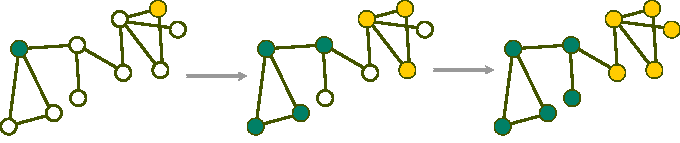
\includegraphics[
                width = 0.85\paperwidth,
                height = 0.85\paperheight,
                keepaspectratio
            ]{images/labelpropagation.pdf}
        \end{center}
        
        \vspace*{0.25cm}
        {\color{darkgray}The algorithm:}
        \begin{columns}[t]
            \column{.50\textwidth}
                \vspace*{-0.1cm}
                \begin{enumerate}
                	\item \small Initially every vertex is labeled with a unique label.
                	\item \small The labels are propagated from vertex to vertex iteratively.
                \end{enumerate}
                
            \column{.50\textwidth}
                \vspace*{-1cm}
                \begin{enumerate}
                    \setcounter{enumi}{2}
                	\item \small At the end of an iteration, each vertex updates its label to the one with maximum weight of neighbor vertices.
                	\item \small Convergence is reached when each vertex is labeled as the majority of its neighbors.
                \end{enumerate}
        \end{columns}
        \note[item]{
            \small Ogni vertice è etichettato con una label unica.
        }
        \note[item]{
            \small Le labels sono fatte propagare da un vertice all'altro in modo iterativo.
        }
        \note[item]{
            \begin{itemize}
                \item \small Alla fine di ogni iterazione di propagazione, un vertice aggiorna la sua label tale che corrisponda a quella col peso massimo dei vertici vicini e loro connessioni.
                \item \small I pareggi sono decisi a random.
            \end{itemize}
        }
        \note[item]{
            \begin{itemize}
                \item \small Si raggiunge un punto di convergenza quando ogni nodo è etichettato come la maggioranza dei suoi vicini.
                \item \small Può succedere che la convergenza ad un'unica soluzione non avvenga in un tempo ragionevole.
                \item \small In tali casi, impostare un numero massimo di iterazioni può essere un trade-off tra accuratezza e tempo d'esecuzione.
            \end{itemize}
            
            {\color{orange}\textbf{This 00:45}} | {\color{red}\textbf{All 08:35}} | {\color{blue}\textit{\large go to next slide}}
        }
    \end{frame}
    
    \begin{frame}{A generic Pregel algorithm}
        
        \hspace*{-0.7cm}
        {\color{darkgray}Pregel's supersteps:}
        \begin{columns}[t]
            \column{.35\textwidth}
                \vspace*{-0.3cm}
                
                \hspace*{-0.1cm}
                {%
                    \color{darkgray}%
                    \small\textbf{Diffusion}: information is propagated from vertex to neighbors.
                }
                
                \hspace*{-0.1cm}
                {%
                    \color{darkgray}%
                    \small\textbf{Fusion}: information is aggregated from neighbors to a set of entities
                }
                
            \column{.65\textwidth}
                \vspace*{-1cm}
                \hspace*{-2cm}
                \begin{center}
                    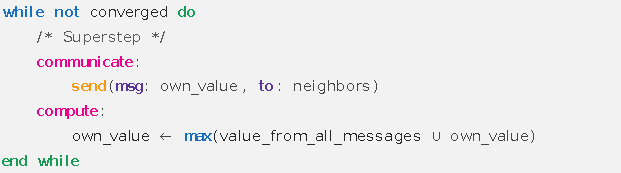
\includegraphics[
                        width = 0.6\paperwidth,
                        height = 0.6\paperheight,
                        keepaspectratio
                    ]{images/pregelpseudocode.pdf}
                \end{center}
                
                \vspace*{-0.1cm}
                \begin{center}
                    \hspace*{-4.7cm}
                    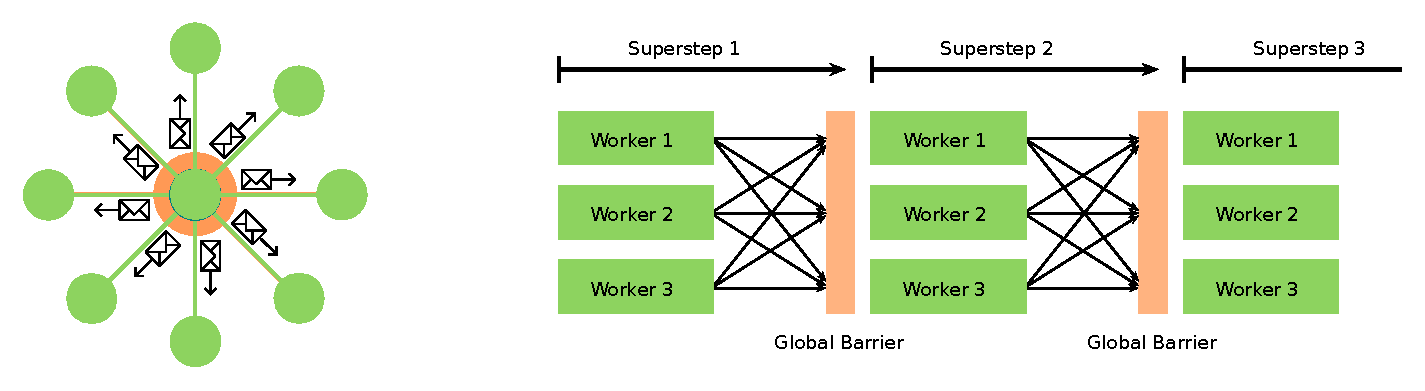
\includegraphics[
                        width = 0.8\paperwidth,
                        height = 0.8\paperheight,
                        keepaspectratio
                    ]{images/ArangoDBCustomPregel2020sendmessage.pdf}
                \end{center}
        \end{columns}
        \note{
            \begin{itemize}
                \item \small Un generico algoritmo Pregel lavora in ambienti distribuiti,
                \item \small con computazioni e dati sparsi in diverse macchine.
            \end{itemize}
            
            \begin{itemize}
                \item \small Per convergere ad uno stato di consenso distribuito,
                \item \small Pregel funziona con iterazioni di superpassi.
            \end{itemize}
            
            \small I superpassi sono due:
        }
        \note[item]{
            \begin{itemize}
                \item \small La fase di diffusione: l'informazione sulle etichette viene propagata da vertice a vertice.
                \item \small Questo step è anche detto di comunicazione del label.
            \end{itemize}
        }
        \note[item]{
            \begin{itemize}
                \item \small L'altra fase è quella di fusione,
                \item \small o di aggregazione dell'informazione dai vertici ad un insieme di nodi.
            \end{itemize}
            
            \large {\color{orange}\textbf{This 00:40}} | {\color{red}\textbf{All 9:15}} | {\color{blue}\textit{Go to next slide}}
        }
    \end{frame}
    
    \begin{frame}{Clustering results}
        \begin{center}
            \vspace*{-0.1cm}
            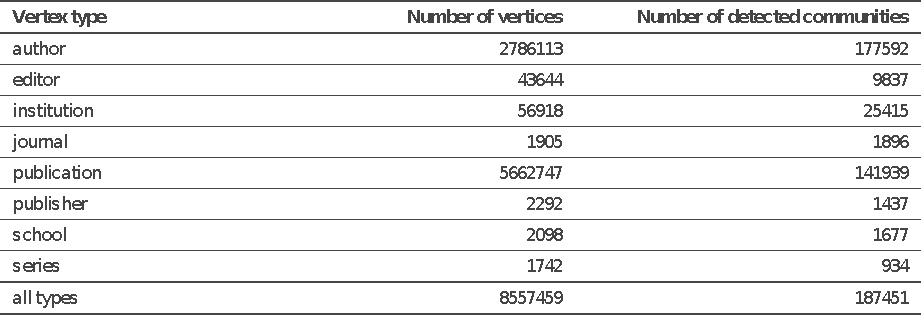
\includegraphics[
                width = 0.85\paperwidth,
                height = 0.85\paperheight,
                keepaspectratio
            ]{images/communitiesdetectedtable.pdf}
        \end{center}
        \note[item]{
            \begin{itemize}
                \item Nel grafo fatto da 8 milioni e mezzo di vertici e 24 milioni di archi,
                \item sono state individuate 187 milla comunità.
            \end{itemize}
        }
        \note[item]{
            \begin{itemize}
                \item Mediamente in una community ci sono 
                \item 16 ricercatori, 2 instituti di affiliazione, 1 journal.
                \item Inoltre, generalmente i nodi di una community hanno fatto mediamente 40 pubblicazioni scientifiche e le pubblicazioni sono associate alla stessa scuola.
            \end{itemize}
            
        }
        \note[item]{
            \begin{itemize}
                \item Per vedere questi risultati in maniare visualmente apprezzabile,
                \item è stata sviluppata una Full-stack Web Application.
                \item Vediamo come è fatta:
            \end{itemize}
            
            {\color{orange}\textbf{This 00:35}} | {\color{red}\textbf{All 09:50}} | {\color{blue}\textit{Go to next slide}}
        }
    \end{frame}
    
    \begin{frame}{Web Application's Architecture}
        \begin{center}
            \vspace*{0.5cm}
            \hspace*{-0.2cm}
            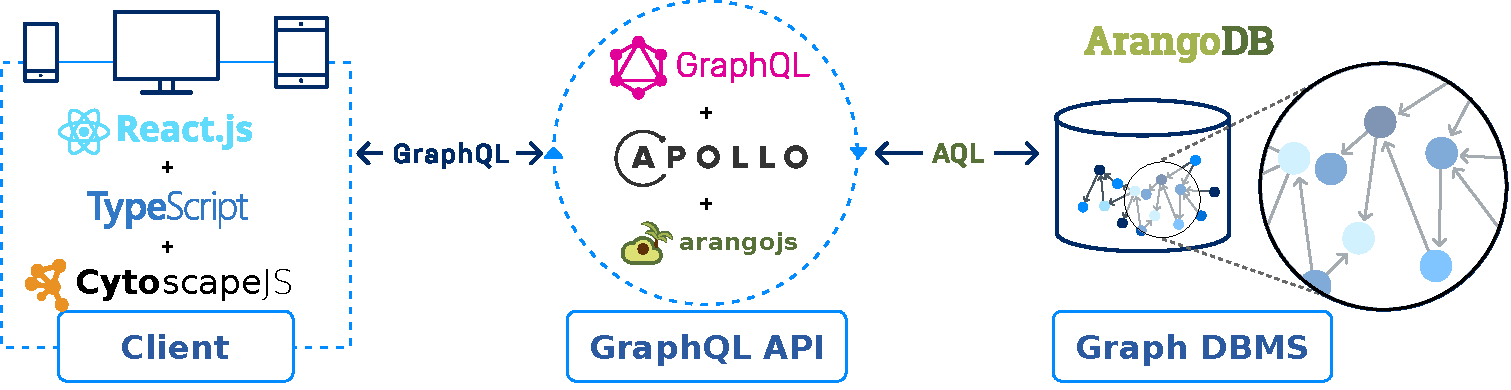
\includegraphics[
                width = 0.9\paperwidth,
                height = 0.9\paperheight,
                keepaspectratio
            ]{images/architecture.pdf}
        \end{center}
        \note[item]{
            \begin{itemize}
                \item \small La Web Application è composta dall'interfaccia lato Frontend
                \item \small e dall'API in backend che fa uso del graph database.
            \end{itemize}
        }
        \note[item]{
            \small Il client è implementato con React, TypeScript e Cytoscape per il rendering dei grafi.
        }
        \note[item]{
            \begin{itemize}
                \item \small L'API è sviluppato con GraphQL ed è servito da Apollo Server.
                \item \small Arangojs è un driver JavaScript che viene usato per comunicare con ArangoDB.
            \end{itemize}
             
        }
        \note[item]{
            \begin{itemize}
                \item \small Il database è ArangoDB, un DBMS multi model, che si presta da graph database.
                \item \small Il linguaggio di querying del database è AQL, ArangoDB Querying Language.
            \end{itemize}
        }
        \note[item]{
            \small 3 macchine servono la WebApp, una per il FE, una per il BE e l'ultima per il DB.
            
            \large {\color{orange}\textit{Wait 10 seconds}}
        }
        \note[item]{
            \begin{itemize}
                \item \small Fino ad ora abbiamo visto la trasformazione dei dati in grafo con ArangoDB.
                \item \small Ora vediamo come è fatto l'API e poi successivamente il frontend.
            \end{itemize}
            
            {\color{orange}\textbf{This 00:50}} | {\color{red}\textbf{All 10:40}} | \large {\color{blue}\textit{Go to next slide}}
        }
    \end{frame}
    
    \begin{frame}{GraphQL API}
        \begin{center}
            
\includegraphics[
                width = 0.85\paperwidth,
                height = 0.85\paperheight,
                keepaspectratio
            ]{images/graphqlapollonew.pdf}
        \end{center}
        \bigskip
        
        {\color{darkgray}The API, initially REST then converted to a GraphQL API, is made of two resolvers:}
        \begin{columns}[t]
            \column{.50\textwidth}
                \begin{enumerate}
                	\item A resolver function to handle the search form autocomplete suggestions.
                \end{enumerate}
                
            \column{.50\textwidth}
                \begin{enumerate}
                    \setcounter{enumi}{1}
                	\item A resolver function to provide collaboration graph's data.
                \end{enumerate}
        \end{columns}
        
        \note[item]{
            \begin{itemize}
                \item Il lato back-end della Web Application, l'API
                \item - è stato sviluppato con NodeJS, Express,
                inizialmente REST API
                \item poi convertito in un GraphQL API con Apollo Server.
            \end{itemize}
        }
        \note[item]{
            \begin{itemize}
                \item GraphQL è un linguaggio di querying e manipolazione dati per APIs.
                \item Fa uso di un sistema a tipi e campi per gestione delle richieste.
            \end{itemize}
            
        }
        \note[item]{
            \begin{itemize}
                \item L'API implementato è composto da due resolver functions.
                \item Uno per la fornire i suggerimenti di autocompletamento durante la ricerca.
                \item L'altro per fornire i dati (vertici, archi e communities)
                \item che compongono il grafo delle collaborazioni.
            \end{itemize}
            
            {\color{orange}\textbf{This 00:35}} | {\color{red}\textbf{All 11:15}} | {\color{blue}\textit{Go to next slide}}
        }
    \end{frame}
    
    \begin{frame}{Frontend UI Layout}
        \begin{center}
            \vspace*{0.5cm}
            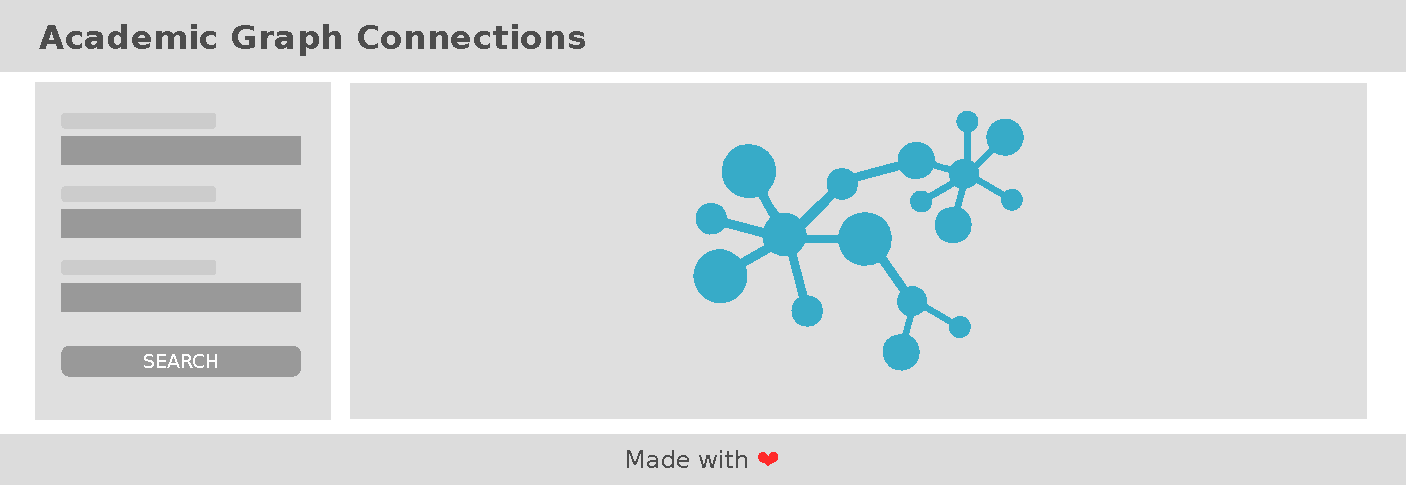
\includegraphics[
                width = 0.85\paperwidth,
                height = 0.85\paperheight,
                keepaspectratio
            ]{images/frontendlayout.pdf}
        \end{center}
        \note[item]{
            \begin{itemize}
                \item La client interface, stilata mediante bootstrap, ha un header,
                \item un content principale suddiviso in due colonne e un footer.
            \end{itemize}
        }
        \note[item]{
            \begin{itemize}
                \item Nella colonna a sinistra del content, l'utente può inserire i dati
                \item per ricercare il grafo delle communità di collaborazione di un nodo.
            \end{itemize}
        }
        \note[item]{
            \begin{itemize}
                \item Nella colonna a destra invece, una volta interrogato l'API
                \item e ricevuta la risposta, viene renderizzato il grafo ricercato.
            \end{itemize}
        }
        \note[item]{
            Vediamo più in dettaglio il form di ricerca.
            
            {\color{orange}\textbf{This 00:35}} | {\color{red}\textbf{All 11:50}} | {\color{blue}\textit{Go to next slide}}
        }
    \end{frame}
    
    \begin{frame}{Frontend UI Search Form}
        \begin{center}
            \vspace*{0.2cm}
            \hspace*{-1cm}
            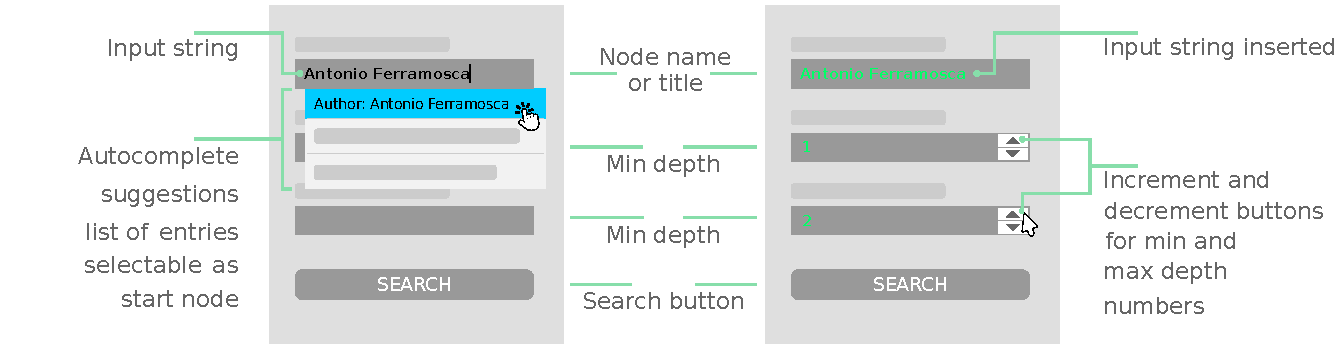
\includegraphics[
                width = 0.95\paperwidth,
                height = 0.95\paperheight,
                keepaspectratio
            ]{images/frontendsearchformautocompletenew.pdf}
        \end{center}
        \note[item]{
            \begin{itemize}
                \item \footnotesize La ricerca è implementata con una feature di autocompletamento
                \item \footnotesize in modo che l'utente possa selezionare un nodo dall'elenco dei nodi suggeriti
                \item \footnotesize e in background il suo nome o titolo verrà tradotto nel suo ID.
                \item \footnotesize Tale ID poi viene usato durante la richiesta del grafo delle collaborazioni.
            \end{itemize}
        }
        \note[item]{
            \begin{itemize}
                \item \footnotesize Nell'esempio mostrato in slide
                \item \footnotesize si è cercato il nodo rappresentante un autore di pubblicazioni scientifiche
                \item \footnotesize di nome "Antonio Ferramosca"
                {\color{orange}\textit{smile}}
            \end{itemize}
        }
        \note[item]{
            \begin{itemize}
                \item \footnotesize Gli altri due campi da compilare sono il minimum e il maximum depth.
                \item \footnotesize Essi rappresentano le distanze minime e massime che i nodi da visualizzare devono avere dal nodo di partenza.
            \end{itemize}
        }
        \note[item]{
            \begin{itemize}
                \item \footnotesize Vediamo un caso concreto.
                \item \footnotesize Ricerchiamo il grafo delle comunità di collaborazione del professor Gargantini.
            \end{itemize}
            
            {\color{orange}\textbf{This 00:55}} | {\color{red}\textbf{All 12:45}} | {\color{blue}\textit{Go to next slide}}
        }
    \end{frame}
    
    \begin{frame}{Results display (Searching for "Angelo Gargantini")}
        \begin{center}
            \vspace*{-0.83cm}
            \hspace*{-1.06cm}
            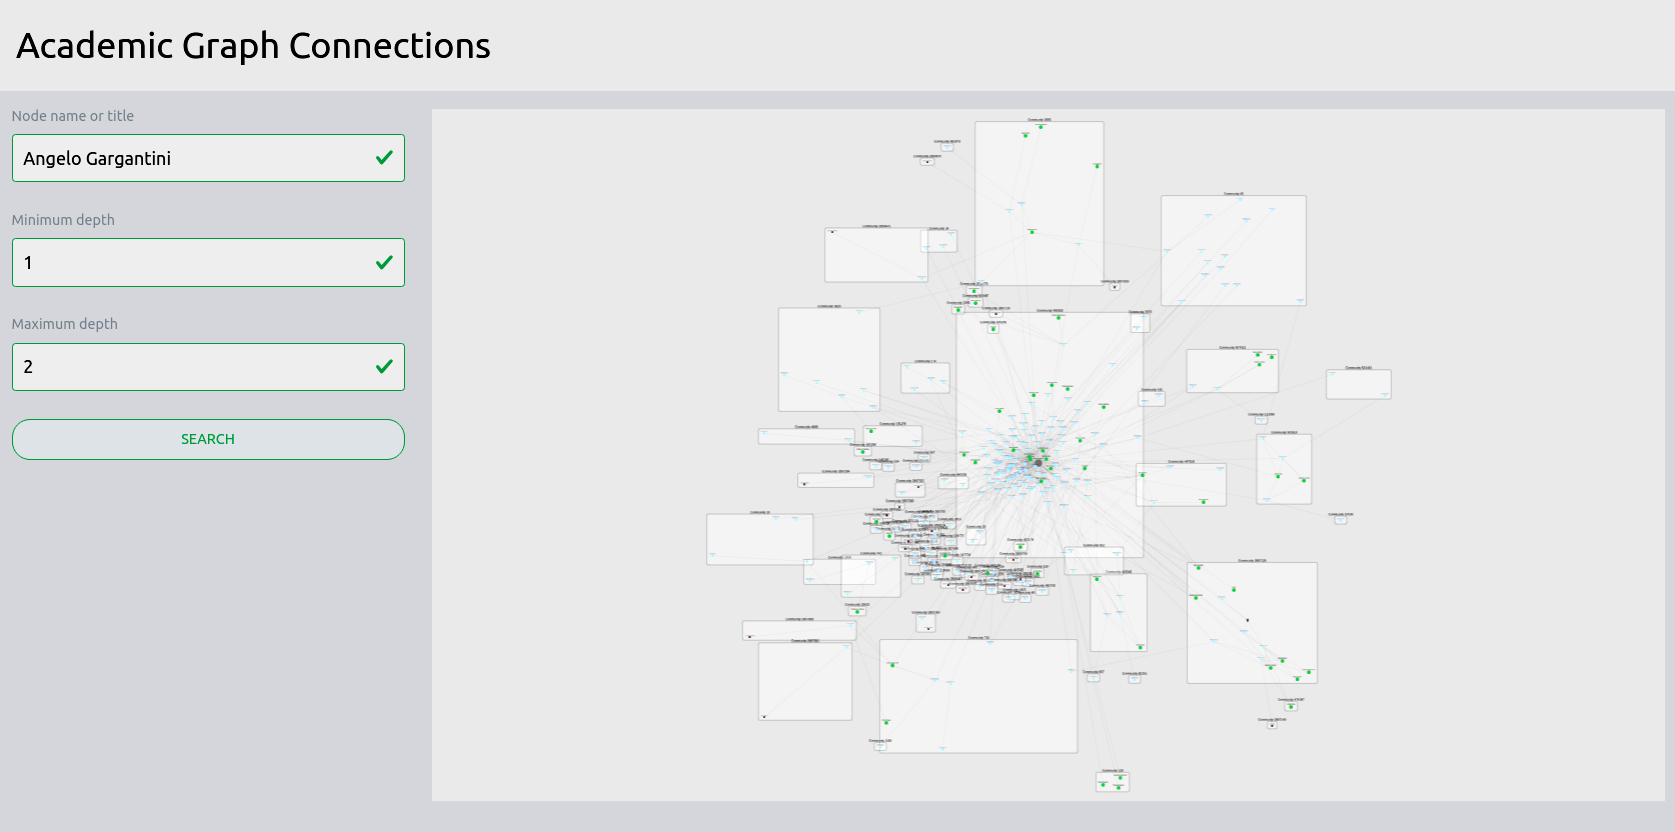
\includegraphics[
                width = 1\paperwidth,
                height = 1\paperheight,
                keepaspectratio
            ]{images/SnapshotLoadedGraphGargantininew.png}
        \end{center}
        \note[item]{
            Nella slide è mostrata l'interfaccia che l'utente vede mentre ricerca il grafo delle communities di collaborazione del professor Gargantini.
        }
        \note[item]{
            A sinistra c'è la sezione dedicata alla ricerca di cui si è parlato nella slide precedente.
        }
        \note[item]{
            \begin{itemize}
                \item A destra invece, una volta finito il querying dell'API
                \item e il fitting dei node e archi del grafo,
                \item viene visualizzato il grafo delle comunità di collaborazione.
            \end{itemize}
        }
        \note[item]{
            \begin{itemize}
                \item È facile notare i rettangoli che rappresentano le communities.
                \item Dentro un rettangolo sono i vertici membri di quella community.
                \item Zoommando in mezzo si può vedere ...
            \end{itemize}
            
            {\color{orange}\textbf{This 00:40}} | {\color{red}\textbf{All 13:25}} | {\color{blue}\textit{Go to next slide}}
        }
    \end{frame}
    
    \begin{frame}{Results display (Angelo Gargantini)}
        \begin{center}
            \vspace*{-0.83cm}
            \hspace*{-1.06cm}
            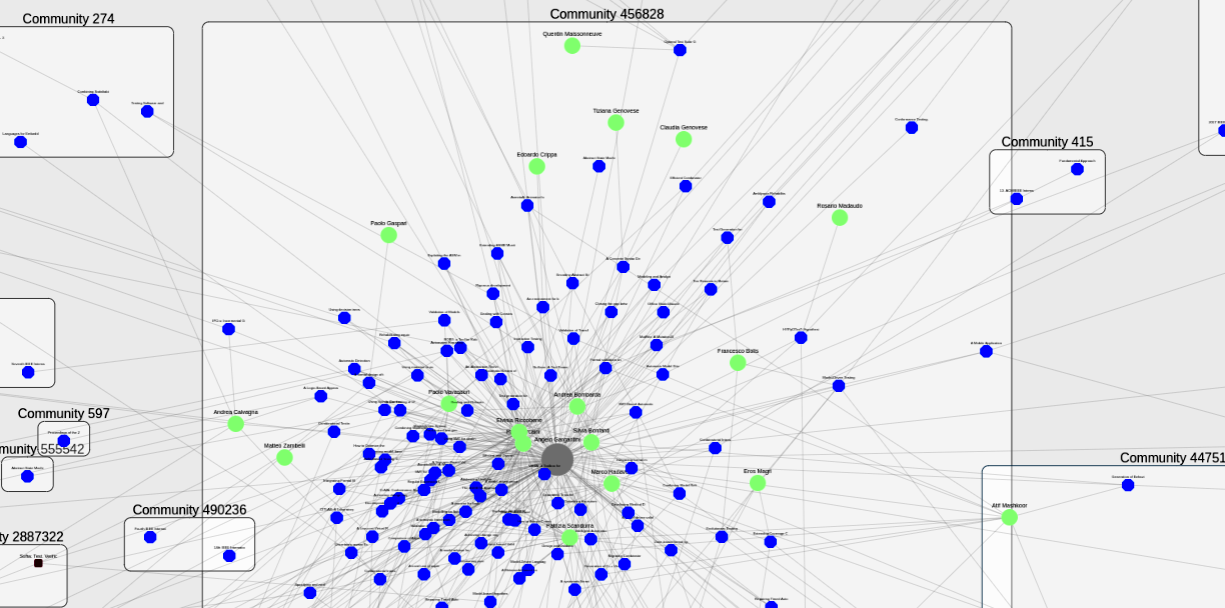
\includegraphics[
                width = 1\paperwidth,
                height = 1\paperheight,
                keepaspectratio
            ]{images/SnapshotLoadedGraphGargantiniZoomnew.png}
        \end{center}
        \note[item]{
            ... come ogni community sia contraddistinta da un ID numerico.
        }
        \note[item]{
            I nodi verdi sono autori, quelli blu sono le pubblicazioni scientifiche.
        }
        \note[item]{
            \begin{itemize}
                \item Un aspetto che può far sorgere dei dubbi
                \item sono le communità mostrate come composte da uno o due nodi.
                \item In realtà esse hanno più nodi, ma perché gli altri nodi distanti dal nodo ricercato, più di un arco, un salto
                \item allora essi non vengono inclusi.
                \item In ogni caso, communità composte da pochi nodi
                \item fanno comunque senso dal punto di vista dell'algoritmo di community detection.
            \end{itemize}
            
            {\color{orange}\textbf{This 00:35}} | {\color{red}\textbf{All 14:00}} | {\color{blue}\textit{Go to next slide}}
        }
    \end{frame}
    
    \begin{frame}{}
        \begin{tikzpicture}[remember picture,overlay]
            \begin{pgfonlayer}{background}
                \node[anchor=south east,outer sep=0pt,inner sep=0pt] at ($(current page.south east) +(-0in,0in)$) {
                    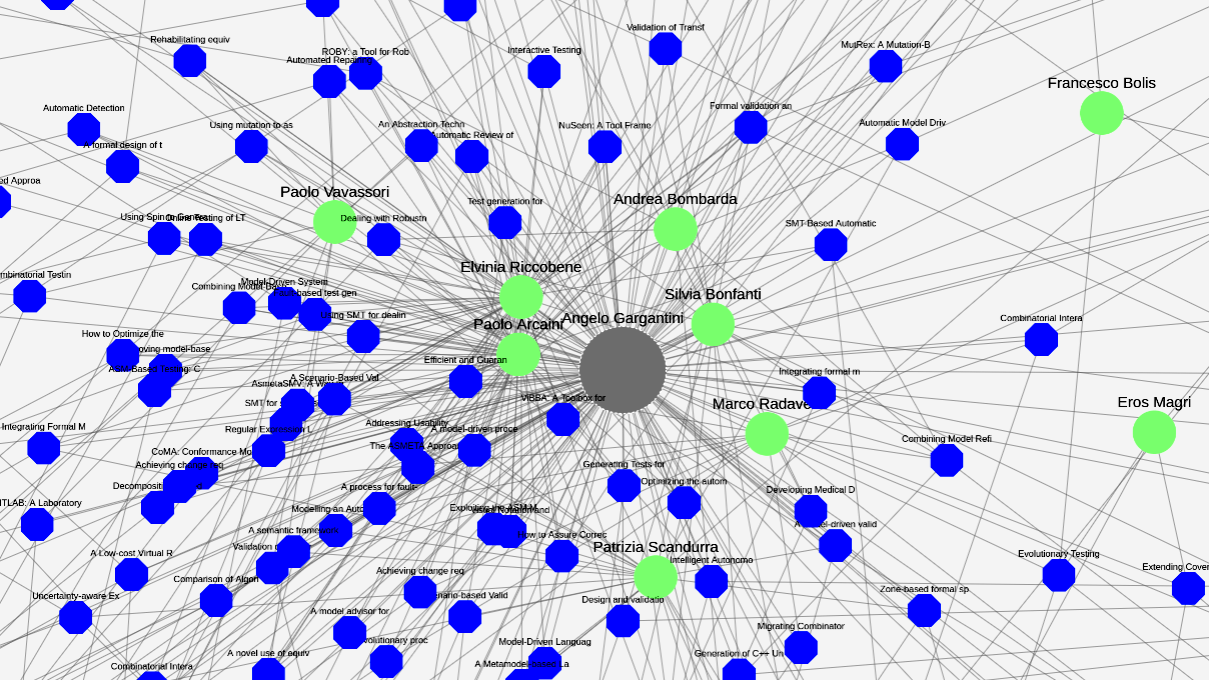
\includegraphics[
                        width = 1\paperwidth,
                        height = 1\paperheight,
                        keepaspectratio
                    ]{images/SnapshotLoadedGraphGargantiniZoomMorenew.png}
                };
            \end{pgfonlayer}
        \end{tikzpicture}
        \note[item]{
            \begin{itemize}
                \item Zoomando ancora, dentro il rettangolo rappresentante la collaboration community,
                \item si possono leggere i nomi dei ricercatori con cui professor Gargantini collabora
                \item e anche i titoli delle pubblicazioni appartenenti a questo cluster.
            \end{itemize}
        }
        \note[item]{
            \begin{itemize}
                \item Uno dei nodi parte del grafo della communità di collaborazione scientifica del professor Gargantini
                \item è anche la professoressa Scandurra.
                \item Se andassimo a ricercare la communità della professoressa ...
            \end{itemize}
            
            {\color{orange}\textbf{This 00:35}} | {\color{red}\textbf{All 14:35}} | {\color{blue}\textit{Go to next slide}}
        }
    \end{frame}
    
    \begin{frame}{Results display (Patrizia Scandurra)}
        \begin{center}
            \vspace*{-0.83cm}
            \hspace*{-1.06cm}
            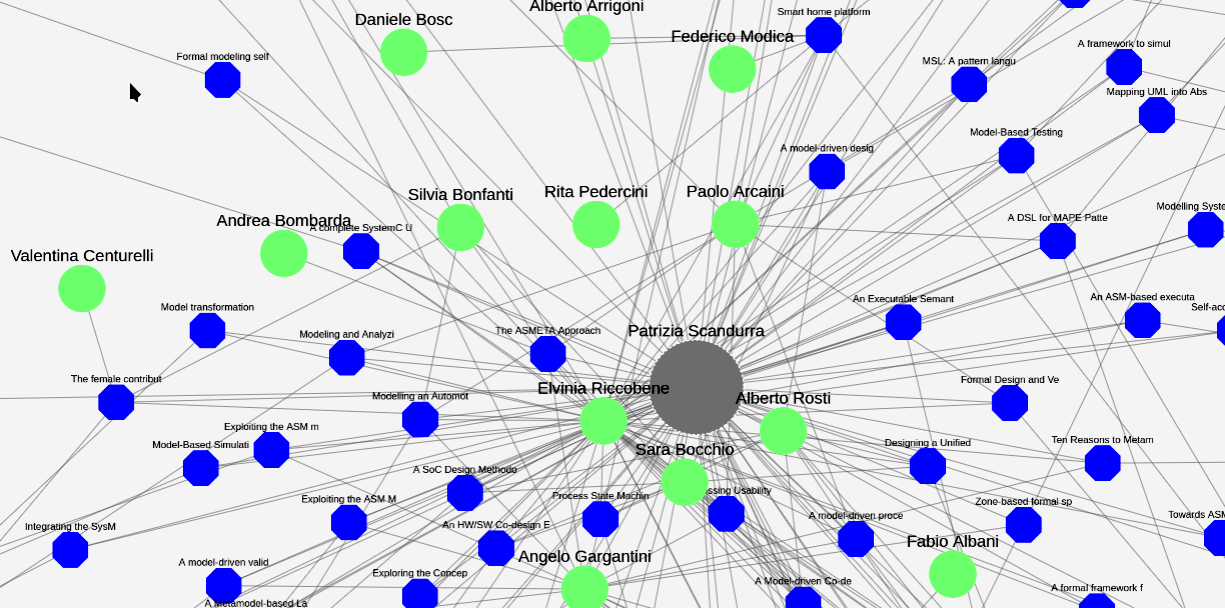
\includegraphics[
                width = 1\paperwidth,
                height = 1\paperheight,
                keepaspectratio
            ]{images/SnapshotLoadedGraphScandurraZoomMorenew.png}
        \end{center}
        \note[item]{
            ... sarebbe possible vedere che la community è la stessa.
        }
        \note[item]{
            \begin{itemize}
                \item Nonostante il posizionamento, il fitting dei nodi sia diverso,
                \item la community è costituita degli stessi nodi e archi.
            \end{itemize}
        }
        \note[item]{
            \begin{itemize}
                \item È interessante far notare che essere docenti nella stessa facoltà e stesso dipartimento,
                \item non necessariamente si traduce in appartenenza alla stessa comunità di collaborazione scientifica.
            \end{itemize}
        }
        \note[item]{
            Ad esempio, cercando il grafo di collaborazione del professor Psaila ...
            
            {\color{orange}\textbf{This 00:35}} | {\color{red}\textbf{All 15:10}} | {\color{blue}\textit{Go to next slide}}
        }
    \end{frame}
    
    \begin{frame}{Results display (Giuseppe Psaila)}
        \begin{center}
            \vspace*{-0.83cm}
            \hspace*{-1.06cm}
            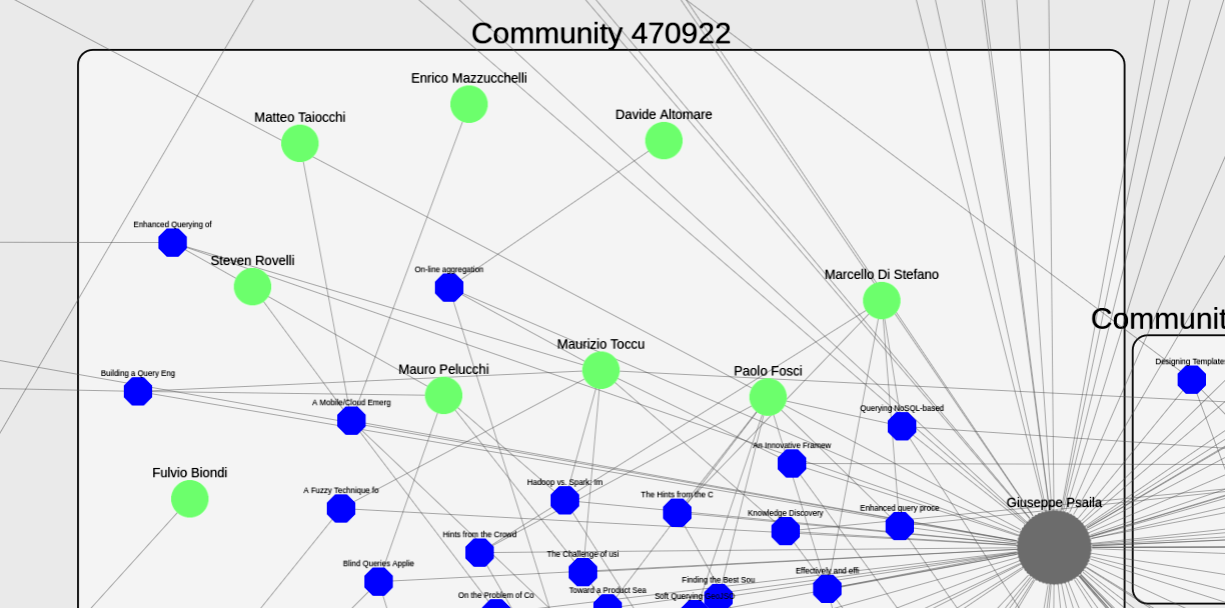
\includegraphics[
                width = 1\paperwidth,
                height = 1\paperheight,
                keepaspectratio
            ]{images/SnapshotLoadedGraphPsailaZoomMorenew.png}
        \end{center}
        \note[item]{
            \begin{itemize}
                \item ... è possibile riconoscere subito i suoi assistenti, Fosci e Pelucchi
                \item ma non sono presenti i docenti visti poc'anzi,
                \item ovvero professor Gargantini o professoressa Scandurra.
            \end{itemize}
        }
        \note[item]{
            \begin{itemize}
                \item Questo succede perché nei dati, di fatto le relazioni (gli archi)
                \item tra loro e il nodo di professor Psaila sono relativamente più sparsi,
                \item meno densi di quanto lo siano con altri ricercatori.
            \end{itemize}
        }
        \note[item]{
            \begin{itemize}
                \item Dal LPA essi quindi vengono individuati, correttamente,
                \item come parte di due comunità di collaborazine scientifica distinte.
            \end{itemize}
        }
        \note[item]{
            Nella successiva slide verrà mostrato il grafo delle comunità di collaborazione accademica ora non più di un autore specifico ... 
            
            {\color{orange}\textbf{This 00:40}} | {\color{red}\textbf{All 15:50}} | {\color{blue}\textit{Go to next slide}}
        }
    \end{frame}
    
    \begin{frame}{Results display (Statistical Methods \& Applications Journal)}
        \begin{center}
            \vspace*{-0.83cm}
            \hspace*{-1.06cm}
            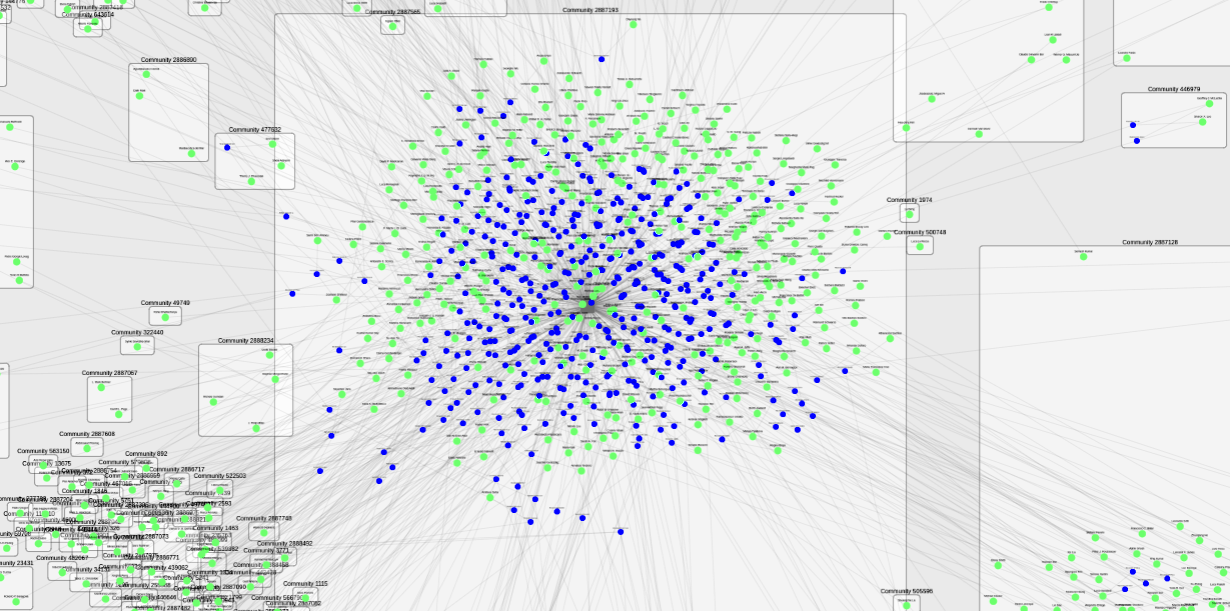
\includegraphics[
                width = 1\paperwidth,
                height = 1\paperheight,
                keepaspectratio
            ]{images/SnapshotLoadedGraphJournalZoomnew.png}
        \end{center}
        \note[item]{
            ... ma di un Journal come quello di Statistical Methods \& Applications.
        }
        \note[item]{
            Uno dei nodi verdi, se zoomassimo, è professor Fassò.
        }
        \note[item]{
            Per concludere ...
            
            {\color{orange}\textbf{This 00:15}} | {\color{red}\textbf{All 16:05}} | {\color{blue}\textit{Go to next slide}}
        }
    \end{frame}
    
    \begin{frame}{Results display (ETH Zurich)}
        \begin{center}
            \vspace*{-0.83cm}
            \hspace*{-1.06cm}
            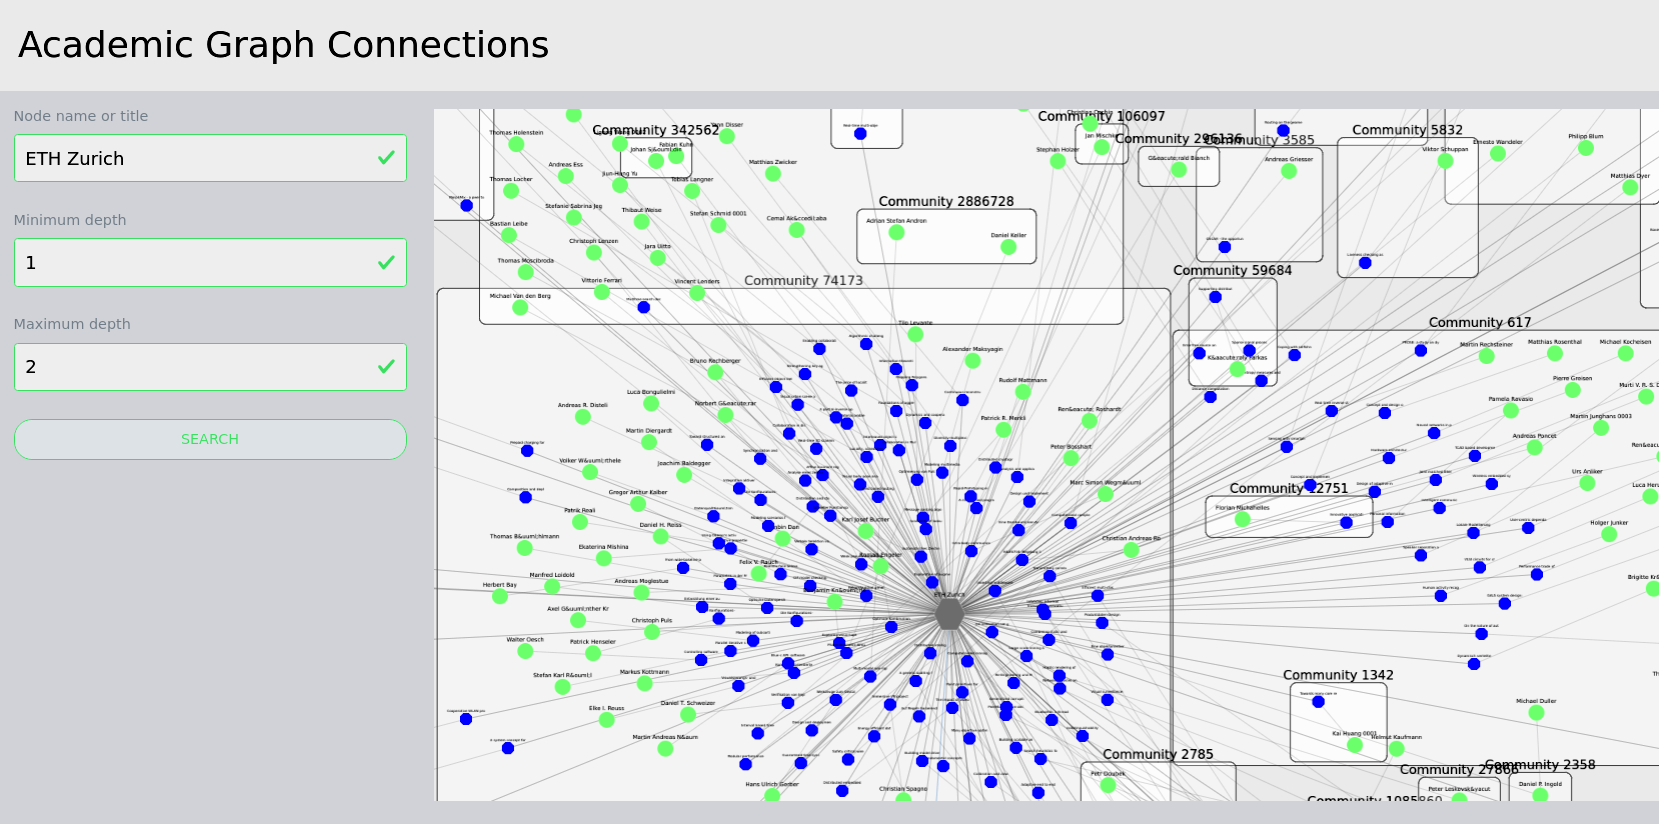
\includegraphics[
                width = 1\paperwidth,
                height = 1\paperheight,
                keepaspectratio
            ]{images/SnapshotLoadedGraphETHZurich12new.png}
        \end{center}
        \note[item]{
            \begin{itemize}
                \item ... a scopo illustrativo della completezza del lavoro svolto,
                \item viene mostra in questa slide come non solo si possano cercare comunità di collaborazione scientifica costruite attorno a ricercatori
                \item o journals, o editors - ma anche communities legate ad una scuola o un istituto accademico di affiliazione.
            \end{itemize}
        }
        \note[item]{
            \begin{itemize}
                \item Nel caso specifico sono mostrate le comunità di collaborazione scientifica della più prestigiosa università di informatica in Europa,
                \item ovvero l'ETH di Zurigo.
            \end{itemize}
        }
        \note[item]{
            Con questa slide finisce la presentazione...
            
            {\color{orange}\textbf{This 00:35}} | {\color{red}\textbf{All 16:40}} | {\color{blue}\textit{Go to next slide}}
        }
    \end{frame}
    
    \begin{frame}[standout]
        \normalfont
        \vspace*{2.25cm}
        \Huge Thank you!
        
        \vspace*{0.625cm}
        Questions?
        
        \vspace*{0.125cm}
        \begin{columns}[t]
            \column{.08\textwidth}
            
            \column{.17\textwidth}
                \vspace*{0.2cm}
                \centering\normalsize\break\myauthor
                
            \column{.25\textwidth}
                \vspace*{-0.9cm}
                \begin{flushright}
                    \large\textbf{\textsc{\break\mydocumenttitle}}
                \end{flushright}
                
            \column{.315\textwidth}
                \vspace*{0.05cm}
                \scriptsize\normalfont\break\mydocumentsubtitle
                
            \column{.10\textwidth}
        \end{columns}
        \note[item]{
            \normalfont
            Grazie mille a tutti per l'attenzione!
        }
        \note[item]{
            \normalfont
            Se avete delle domande...
            
            {\color{orange}\textbf{This 00:20}} | {\color{red}\textbf{All 17:00}} | {\color{orange}\textit{wait for questions}}
        }
    \end{frame}
    \stepcounter{framenumber}
\end{document}
